\documentclass[lettersize,journal]{IEEEtran}
\usepackage{amsmath,amsfonts,amssymb}
% \usepackage{algorithmic}
\usepackage{algorithm}
\usepackage{algpseudocode}
\usepackage{array}
\usepackage[caption=false,font=normalsize,labelfont=sf,textfont=sf]{subfig}
\usepackage{textcomp}
\usepackage{stfloats}
\usepackage{url}
\usepackage{verbatim}
\usepackage{graphicx}
\usepackage{cite}
\hyphenation{op-tical net-works semi-conduc-tor IEEE-Xplore}
% updated with editorial comments 8/9/2021
\usepackage{booktabs}
\usepackage{tikz}          
\usepackage{varwidth} % tikz
\usetikzlibrary{positioning, shapes.geometric} % tikz
\usepackage[T1]{fontenc}
\usepackage[utf8]{inputenc}
\usepackage{xcolor,colortbl}
\graphicspath{ {images/} } 
\usepackage{blindtext}
% \usepackage{subfiles}
% \usepackage{subcaption}
\usepackage{multicol}
% \usepackage{stfloats}
\usepackage{array}
\usepackage{caption}
\usepackage{url}
\usepackage{cite}
\usepackage{adjustbox}
\usepackage[dvipsnames]{xcolor}
\usepackage{placeins}
% \usepackage{subcaption}
% \usepackage{subfigure}
\newcolumntype{C}[1]{>{\centering\arraybackslash}p{#1}}
\newcolumntype{M}[1]{>{\centering\arraybackslash}m{#1}}
\usepackage{subfig}
\usepackage{amsthm}
\usepackage{needspace} 
\usepackage{amssymb}
\newtheorem{lemma}{Lemma}
\newtheorem{problem}{Problem}
\newtheorem*{problem*}{Problem}
\newtheorem{proposition}{Proposition}
\newcommand{\mycomment}[1]{}
\newcommand{\algrule}[1][.2pt]{\par\vskip.5\baselineskip\hrule height #1\par\vskip.5\baselineskip}



\begin{document}


\title{A Graph-Based Approach to the Topological Optimization of Cycling Networks for the Improvement of Safety and Comfort of Cyclists}




\author{Manuel Campero Jurado$^{1}$, Carlos Canudas-de-Wit$^{2}$,  Giovanni De Nunzio$^{3}$% <-this % stops a space
%\thanks{*This work was not supported by any organization}% <-this % stops a space
\thanks{$^{1}$Univ. Grenoble Alpes, Inria, 38334 Montbonnot Cedex - France 
        {\footnotesize manuel.campero-jurado@inria.fr} (\textit{Corresponding author})}%
\thanks{$^{2}$Univ. Grenoble Alpes, CNRS, Inria, Grenoble INP, GIPSA-lab, 11 Rue des Mathématiques, 
38400 Saint-Martin-d'Hères-Grenoble-France
        {\footnotesize carlos.canudas-de-wit@gipsa-lab.fr}}%
\thanks{$^{3}$IFP Energies nouvelles,
Rond-point de l’échangeur de Solaize, BP 3, 69360 Solaize, France,
        {\footnotesize giovanni.de-nunzio@ifpen.fr}}%
}

% The paper headers
%\markboth{Journal of \LaTeX\ Class Files,~Vol.~14, No.~8, August~2021}%
%{Shell \MakeLowercase{\textit{et al.}}: A Sample Article Using IEEEtran.cls for IEEE Journals}

%\IEEEpubid{0000--0000/00\$00.00~\copyright~2021 IEEE}
% Remember, if you use this you must call \IEEEpubidadjcol in the second
% column for its text to clear the IEEEpubid mark.

\maketitle

\begin{abstract}


This work aims to improve perceived safety and comfort of cyclists by proposing a topological optimization of existing cycling networks. We assign weights to a six-category system for bike lanes based on their segregation from motorized vehicles using the well-developed CycleRAP tool. Each bike lane is weighted based on its category and topological features. Graph theory metrics are then applied to analyze the core topological characteristics of cycling networks across various French municipalities. These metrics form the basis for estimating and predicting cyclists' perceived safety and comfort levels, as reported in local surveys. Building on this relationship, we formulate a topology optimization problem aimed at maximizing predicted safety and comfort within budgetary constraints. To tackle this complex problem, we introduce a topological optimization algorithm and compare its performance with existing algorithms to ensure reliability. This approach integrates graph theory with real-world indicators, providing a comprehensive quantitative framework to support decision-making in urban planning and resource allocation.


\end{abstract}


\begin{IEEEkeywords}
Cycling network, graph theory,  safety, comfort, budget-constrained infrastructure optimization, heuristic optimization.
\end{IEEEkeywords}

\section{INTRODUCTION}


% The health, ecological, and socio-economic benefits of a cyclist society are well-known, including improved cardiovascular health, increased longevity, reduced carbon footprint, decreased air pollution, lower transportation costs, reduced traffic congestion, and greater convenience and efficiency \cite{garrard2012health, krizec2007estimating, gotschi2016cycling}. As a result, public authorities have made considerable efforts to promote cycling as an alternative to driving for short distances, however, cyclists continue to face safety and comfort issues that may dissuade them from cycling \cite{fishman2012barriers}. It is well-established that infrastructure separating bicycles from motorized vehicles improves user perceptions of safety and comfort, encouraging increased cycling \cite{lawrence2018cyclist, broach2012cyclists}. High-quality cycling infrastructure has a significant impact on ridership, with great potential for growth when there are highly connected facilities \cite{pucher2011walking, pucher2017cycling}. Given the often limited budget for infrastructure development, it is crucial to determine where to allocate resources to maximize the impact on cyclists' safety and comfort. This work presents a cycling network classification weighted using the international assessment tool CycleRAP \cite{cyclerap2024}. Additionally, it proposes a modeling and optimization framework to identify the most effective bike lane upgrades for enhancing cyclist safety and comfort
% Cycling offers well-known health, ecological, and socio-economic benefits, including improved health, reduced emissions, lower costs, and less traffic congestion \cite{garrard2012health, krizec2007estimating, gotschi2016cycling}. Despite efforts to promote cycling, safety and comfort concerns remain major barriers \cite{fishman2012barriers}. Infrastructure that separates cyclists from motorized vehicles significantly improves perceptions of safety and boosts ridership \cite{lawrence2018cyclist, broach2012cyclists}. With limited budgets for development, strategic resource allocation is essential. This work classifies cycling networks using CycleRAP \cite{cyclerap2024} and introduces an optimization framework to prioritize bike lane upgrades for safety and comfort.
% The benefits of cycling society are well-known, including better cardiovascular health, longer life, reduced carbon footprint, lower air pollution, lower transportation costs, less traffic congestion, and increased efficiency \cite{garrard2012health, gotschi2016cycling}. Public authorities have promoted cycling as an alternative to driving for short trips, but cyclists still face safety and comfort issues \cite{fishman2012barriers}. Infrastructure that separates bikes from motor vehicles improves perceptions of safety, boosting cycling \cite{lawrence2018cyclist, broach2012cyclists}. High-quality cycling infrastructure significantly impacts ridership, especially when networks are highly connected \cite{pucher2011walking, pucher2017cycling}. With limited budgets for infrastructure, it is essential to allocate resources effectively to improve safety and comfort. This work introduces a cycling network classification based on the CycleRAP tool \cite{cyclerap2024} and proposes an optimization framework to identify the most effective bike lane upgrades for safety and comfort
The health, ecological, and socio-economic benefits of a cyclist society are well-known, including improved cardiovascular health, increased longevity, reduced carbon footprint, decreased air pollution, lower transportation costs, reduced traffic congestion, and greater convenience and efficiency \cite{garrard2012health, gotschi2016cycling}. As a result, public authorities have made considerable efforts to promote cycling as an alternative to driving for short distances, however, cyclists continue to face safety and comfort issues that may dissuade them from cycling \cite{fishman2012barriers}. It is well-established that infrastructure separating bicycles from motorized vehicles improves user perceptions of safety and comfort, encouraging increased cycling \cite{lawrence2018cyclist, broach2012cyclists}. High-quality cycling infrastructure has a significant impact on ridership, with great potential for growth when there are highly connected facilities \cite{pucher2011walking, pucher2017cycling}. Given the often limited budget for infrastructure development, it is crucial to determine where to allocate resources to maximize the impact on cyclists' safety and comfort. This work presents a cycling network classification weighted using the international assessment tool CycleRAP \cite{cyclerap2024}. Additionally, it proposes a modeling and optimization framework to identify the most effective bike lane upgrades for enhancing cyclist safety and comfort.



\subsection{Literature Review} 
Our work pertains to three research streams: safety and comfort levels in cycling networks, optimization of cycling infrastructure, and the application of graph theory metrics to evaluate transportation network characteristics.


% Various frameworks have been developed to classify roads and paths in cycling networks based on safety and comfort. One widely adopted framework is the Levels of Traffic Stress (LTS), which categorizes roads into four levels depending on infrastructure characteristics such as protected lanes, speed limits, and traffic volume \cite{crist2019fear}. Additionally, models like the Bicycle Safety Index Rating (BSIR) assess subjective perceptions of road safety, while the Bicycle Level of Service (BLOS) index evaluates ride comfort and traffic conditions \cite{bian2021categorizing, campisi2020cycling}. Another tool, the Bicycle Environmental Quality Index, considers broader factors such as intersection safety, street design, and land use.

% These frameworks often depend on the local context and user perception, emphasizing the importance of tailoring assessments to specific locations \cite{boettge2017assessing}. 

% However, the previous categories are usually based on data and surveys that are not transferable to all regions, that is why we adopt a six-category classification system for bike lanes based on their segregation from motorized vehicles, referred to as the degree of separation (DoS)  that relies entirely on OpenStreetMap (OSM) data \cite{2024graphbased}, thus completely generalizable. In this system, greater segregation correlates with higher levels of safety and comfort. 
\textit{Safety and Comfort Levels in Cycling Networks}: Several frameworks classify cycling network roads and paths by safety and comfort. The Levels of Traffic Stress (LTS) categorize roads into four levels based on infrastructure like protected lanes, speed limits, and traffic volume \cite{crist2019fear}. Additionally, models like the Bicycle Safety Index Rating (BSIR) assess subjective perceptions of road safety, while the Bicycle Level of Service (BLOS) index evaluates ride comfort and traffic conditions \cite{bian2021categorizing, campisi2020cycling}.

% These frameworks highlight the need for location-specific assessments, as they depend heavily on local data and user perception \cite{boettge2017assessing}. To ensure generalizability, we adopt a six-category classification system for bike lanes based on their degree of separation (DoS) from motorized vehicles, relying solely on OpenStreetMap (OSM) data \cite{2024graphbased}, where greater segregation indicates higher safety and comfort.

% These frameworks often depend on the local context and user perception, emphasizing the importance of tailoring assessments to specific locations \cite{boettge2017assessing}. 

However, the previous categories are usually based on data and surveys that are not transferable to all regions, that is why we adopt a six-category classification system for bike lanes based on their segregation from motorized vehicles, referred to as the degree of separation (DoS)  that relies entirely on OpenStreetMap (OSM) data \cite{2024graphbased}, thus completely generalizable. In this system, greater segregation correlates with higher levels of safety and comfort. 


% The Bicycle Network Improvement Problem (BNIP) formalizes network enhancement by selecting road upgrades to maximize safety and reduce route deviations within a budget. 

% Design principles for cycling infrastructure prioritize safety through features such as protected lanes, sufficient path widths, and buffer zones from motorized traffic. Enhancing comfort involves minimizing interruptions and ensuring smooth, direct routes \cite{schroter2021guidance, nesmachnow2024assessment}. Metrics like the Level of Traffic Stress (LTS) and Bicycle Compatibility Index (BCI) are frequently used to assess infrastructure effectiveness and user satisfaction \cite{crist2019fear, campisi2020cycling}. Specific optimization approaches vary, with some focusing on maximizing the travel distance covered on designated bike lanes, which refers to increasing the total distance that cyclists travel on designated bike lanes, a metric used as a proxy for improved infrastructure usage and accessibility  \cite{mesbah2012bilevel, smith2012mathematical}, while others emphasize improving connectivity and societal benefit-cost ratios within budget constraints \cite{paulsen2023societally, duthie2014optimization}. Mixed-integer programming and metaheuristics have also been employed to design reliable urban networks that balance user preferences and economic feasibility \cite{mauttone2017bicycle}.  This problem has been modeled as a Mixed-Integer Linear Program (MIP) and solved with scalable Benders decomposition, validated on real-world data \cite{lim2022bicycle}. Similarly, bikeway optimization models often minimize travel time under budget constraints, with genetic algorithms and heuristics proving effective \cite{shui2019optimization}. Demand-driven approaches that integrate car and bike networks enable resource reallocation for maximum impact \cite{steinacker2022demand}..

% In \cite{paulsen2023societally}, the expansion of cycling networks is examined by maximizing the societal benefit-cost ratio of adding bicycle infrastructure, weighing anticipated benefits against construction and maintenance costs to evaluate economic feasibility. Another strategy aims to enhance network graph connectivity. For instance, \cite{duthie2014optimization} proposes an optimization framework that minimizes the cost of network improvements by enhancing connectivity, ensuring all origin-destination pairs are linked with paths that meet specified criteria for cycling level of service. Similarly, \cite{mauttone2017bicycle} presents an optimization framework for urban bicycle network design that balances user preferences for shortest paths with planners' budget constraints. A mixed-integer mathematical program is used to account for user costs on segments lacking cycling infrastructure, and a metaheuristic is applied to large networks to minimize route discontinuities.
 
% While these methods show potential, there remains a critical gap in systematically validating whether the proposed changes align with real-world perceptions of safety and comfort, as reflected in survey data.

% \textit{Cycling Network Optimization}: The Bicycle Network Improvement Problem (BNIP) focuses on upgrading roads to maximize safety and reduce route deviations within budget constraints. Key principles include protected lanes, sufficient path widths, and smooth, direct routes to enhance safety and comfort \cite{schroter2021guidance, nesmachnow2024assessment}. Metrics like the LTS and Bicycle Compatibility Index (BCI) assess infrastructure effectiveness \cite{crist2019fear, campisi2020cycling}.

% Optimization approaches range from maximizing travel distance on bike lanes \cite{mesbah2012bilevel, smith2012mathematical} which refers to increasing the total distance that cyclists travel on designated bike lanes, a metric used as a proxy for improved infrastructure usage and accessibility. For improving connectivity and societal benefit-cost ratios \cite{paulsen2023societally, duthie2014optimization}. Mixed-integer programming and metaheuristics have been used for reliable urban networks, balancing user preferences and costs \cite{mauttone2017bicycle, lim2022bicycle}. Genetic algorithms and heuristics effectively minimize travel time under budget constraints \cite{shui2019optimization}, while demand-driven models integrate car and bike networks for resource reallocation \cite{steinacker2022demand}.

% Strategies also enhance network connectivity, ensuring origin-destination pairs meet service criteria \cite{duthie2014optimization}, or balance shortest paths with budget constraints using mixed-integer models \cite{mauttone2017bicycle}. Although promising, these methods often lack validation against real-world perceptions of safety and comfort from survey data.
  \textit{Cycling Network Optimization}: Numerous studies explore different aspects of cycling network topology optimization, this includes upgrading specific bike lanes to achieve the dual goals of improved safety and comfort, all while adhering to resource constraints. The Bicycle Network Improvement Problem (BNIP) aims to enhance safety and reduce route deviations while staying within budget constraints. Key considerations include protected lanes, sufficient path widths, and direct routes \cite{schroter2021guidance, nesmachnow2024assessment}. These factors are typically assessed using metrics such as the LTS and the Bicycle Compatibility Index (BCI) \cite{crist2019fear, campisi2020cycling}.
% There is an extensive amount of works in optimizing cycling networks for example the Bicycle Network Improvement Problem (BNIP) aims to enhance safety and minimize route deviations within budget constraints. Key factors include protected lanes, sufficient path widths, and direct routes \cite{schroter2021guidance, nesmachnow2024assessment}, assessed using metrics like LTS and Bicycle Compatibility Index (BCI) \cite{crist2019fear, campisi2020cycling}.

% Optimization strategies maximize bike lane usage \cite{mesbah2012bilevel, smith2012mathematical} which refers to increasing the total distance that cyclists travel on designated bike lanes, a metric used as a proxy for improved infrastructure usage and accessibility. Also are studies for improving connectivity and societal benefit-cost ratios \cite{paulsen2023societally, duthie2014optimization}. Additionally, demand-driven models integrate car and bike networks for resource reallocation \cite{steinacker2022demand}, while others prioritize connectivity or budget-aware shortest paths \cite{duthie2014optimization}. And people have used mixed-integer programming and metaheuristics for finding reliable urban networks, balancing user preferences and costs \cite{mauttone2017bicycle, lim2022bicycle}. Genetic algorithms and heuristics effectively minimize travel time under budget constraints \cite{shui2019optimization}. Although promising, these methods often lack validation against real-world perceptions of safety and comfort from survey data.

Optimization strategies maximize bike lane usage \cite{mesbah2012bilevel, smith2012mathematical} which refers to increasing the total distance that cyclists travel on designated bike lanes, a metric used as a proxy for improved infrastructure usage and accessibility.  Other studies emphasize improving network connectivity and optimizing societal benefit-cost ratios \cite{paulsen2023societally, duthie2014optimization}. Demand-driven models integrate car and bike networks to guide resource reallocation \cite{steinacker2022demand}, while some approaches prioritize connectivity or budget-aware shortest paths \cite{duthie2014optimization}. Mixed-integer programming and metaheuristic approaches have been applied to optimize urban cycling networks, balancing user preferences and costs \cite{mauttone2017bicycle, lim2022bicycle}. Additionally, genetic algorithms and heuristics have been used to minimize travel time while adhering to budget constraints \cite{shui2019optimization}. Despite their potential, these methods often lack validation against real-world perceptions of safety and comfort derived from survey data.


% Graph theory metrics offer valuable insights into the analysis and optimization of transportation networks. Key metrics include betweenness centrality, which identifies critical nodes based on shortest path traversal \cite{dees2021graph}, and algebraic connectivity, which assesses network robustness using the second smallest eigenvalue of the Laplacian matrix \cite{elaraby2021connectivity}. Other metrics, such as the spectral radius, measure communication efficiency within the network \cite{di2018applications}, while modularity and community structure detect clusters or modules, aiding in targeted interventions \cite{elaraby2021connectivity}. These metrics help quantify connectivity, efficiency, and resilience, providing a robust foundation for network analysis.

% Resilience in transport networks can also be evaluated using connectivity measures, with algebraic connectivity particularly sensitive to topological changes \cite{yang2016rationality}. The characteristic path length, which reflects the average shortest paths in a network, provides guidance for infrastructure improvement \cite{sydney2010characterising}. Applications of these metrics in cycling networks have demonstrated their utility in prioritizing upgrades on critical paths, minimizing vulnerabilities, and ensuring equitable access across diverse regions \cite{araujo2000function}. By integrating these tools into optimization frameworks, researchers and planners can achieve safer and more comfortable cycling networks while addressing challenges related to efficiency and fairness.

%   Other approaches utilize graph-theoretical tools. For instance, studies such as \cite{kamel2021impact, akbarzadeh2018designing} explore the relationship between graph theory metrics and bike-vehicle traffic and propose bike network design strategies based on network clustering. However, all their approaches often assume that changes to bike lane topology will consistently improve these metrics, overlooking the complex and non-monotonic nature of graph theory metrics. 
  
% This study adopts the DoS category proposed in \cite{2024graphbased}, which utilizes OSM data to assign linear weights to roads based on their DoS. Using this approach, the authors apply graph theory metrics to examine the core topological features of cycling networks in eleven municipalities across France. These metrics are assessed to identify those that effectively indicate and predict cyclists' perceived safety and comfort levels, as captured through survey data.

% It is important to note that the available survey data on perceived safety and comfort is aggregated at a regional level, meaning there is not safety or comfort detailed information at the level of individual streets or links. Therefore, the proposed analysis and methods focus on broader regional trends, assessing how local modifications influence the overall safety and comfort of the network.

% Building on this relationship, they propose a topology optimization framework aimed at enhancing perceived safety and comfort while adhering to budget constraints. This involves improving the structure of the cycling network by modifying its topology such as upgrading specific bike lanes based on graph theory metrics to achieve the dual objectives of improved safety and comfort while staying within resource limitations.


% Nevertheless, using linear weights for the graph edges may not accurately reflect the complexities of real-world bike networks, where weights are often non-linear due to diverse and intricate topological characteristics. Additionally, the criteria for selecting metrics that effectively predict perceived safety and comfort are not clearly defined, creating uncertainty about their predictive accuracy. Furthermore, the proposed optimization algorithm solver is not benchmarked against established algorithms, making it challenging to evaluate its practical utility and effectiveness.
% \textit{Graph Theory Metrics in Cycling Networks}: Graph theory metrics provide critical insights for analyzing and optimizing transport networks. Betweenness centrality identifies crucial nodes on shortest paths \cite{dees2021graph}, while algebraic connectivity assesses robustness via the second smallest Laplacian eigenvalue \cite{elaraby2021connectivity}. Spectral radius measures communication efficiency \cite{di2018applications}, and modularity detects network clusters for targeted interventions \cite{elaraby2021connectivity}. These metrics quantify connectivity, efficiency, and resilience, offering valuable tools for network improvement and enhancements like utility in prioritizing upgrades on critical paths, minimizing vulnerabilities, and ensuring equitable access across diverse regions \cite{yang2016rationality, sydney2010characterising, araujo2000function}. Other approaches utilize graph-theoretical tools, for instance, studies such as \cite{kamel2021impact, akbarzadeh2018designing} explore the relationship between graph theory metrics and bike-vehicle traffic and propose bike network design strategies based on network clustering.

\textit{Graph Theory Metrics in Cycling Networks}:  
Graph theory metrics offer valuable tools for analyzing and optimizing transport networks. Betweenness centrality identifies key nodes along shortest paths, highlighting critical infrastructure points \cite{dees2021graph}. Algebraic connectivity, measured by the second smallest Laplacian eigenvalue, assesses network robustness \cite{elaraby2021connectivity}, while spectral radius evaluates communication efficiency \cite{di2018applications}. Modularity helps detect network clusters, facilitating targeted interventions \cite{elaraby2021connectivity}. These metrics collectively quantify connectivity, efficiency, and resilience, aiding in network improvements such as prioritizing upgrades on critical paths, minimizing vulnerabilities, and promoting equitable access across diverse regions \cite{yang2016rationality, sydney2010characterising, araujo2000function}. Additionally, graph-theoretical approaches have been used to study bike-vehicle interactions and develop network design strategies based on clustering \cite{kamel2021impact, akbarzadeh2018designing}. However, all their approaches often assume that changes to bike lane topology will consistently improve these metrics, overlooking the complex and non-monotonic nature of graph theory metrics. 

%   Other approaches utilize graph-theoretical tools. For instance, studies such as \cite{kamel2021impact, akbarzadeh2018designing} explore the relationship between graph theory metrics and bike-vehicle traffic and propose bike network design strategies based on network clustering. However, all their approaches often assume that changes to bike lane topology will consistently improve these metrics, overlooking the complex and non-monotonic nature of graph theory metrics. 

To the best of our knowledge, no existing work systematically integrates globally aggregated graph theory metric values into a robust weighting framework for modeling perceived cycling safety and comfort.
Additionally, current optimization approaches lack rigorous benchmarking against state-of-the-art algorithms. This work bridges these gaps by introducing a refined weighting methodology and systematically evaluating its optimization framework.

% To the best of the authors' knowledge, no existing work provides a well-justified weighting framework for modeling safety and comfort using graph theory metrics or systematically benchmarks optimization frameworks. This work addresses these gaps by introducing a refined weighting methodology and rigorously evaluating its optimization framework against state-of-the-art methods.  

% Existing approaches often assume that modifications to bike lane topology will consistently improve key metrics, overlooking the non-monotonic nature of graph theory metrics. Additionally, current methods rely on linear edge weights that may not accurately capture the complexities of real-world cycling networks, where weights are often nonlinear due to diverse topological characteristics. Furthermore, the selection criteria for predictive metrics remain unclear, and optimization frameworks lack benchmarking against established algorithms, making their reliability and practical utility uncertain.  

% To the best of the authors' knowledge, there is no well-justified weighting framework for modeling safety and comfort in cycling networks using graph theory metrics. Additionally, no prior work has systematically benchmarked optimization frameworks against established algorithms to validate their effectiveness. This work addresses these gaps by introducing a more robust weighting methodology tailored to real-world cycling networks and proposing an optimization framework that is rigorously evaluated against state-of-the-art methods.

% However, all their approaches often assume that changes to bike lane topology will consistently improve these metrics, overlooking the complex and non-monotonic nature of graph theory metrics. So, using the DoS framework from \cite{2024graphbased}, which assigns weights based on OSM data, graph metrics with monotonic properties are applied to analyze cycling networks in 11 French municipalities. These metrics predict cyclists' perceived safety and comfort levels from aggregated survey data. However, using linear weights for the graph edges may not accurately reflect the complexities of real-world bike networks, where weights are often non-linear due to diverse and intricate topological characteristics. Additionally, the criteria for selecting metrics that effectively predict perceived safety and comfort are not clearly defined, creating uncertainty about their predictive accuracy. Furthermore, the proposed optimization algorithm solver is not benchmarked against established algorithms, making it challenging to evaluate its practical utility and effectiveness. In conclusion, to the best of the authors' knowledge, there is a lack of well justified weithed for bike lanes for modeling safety and comfort with graph theory metric and lack of optimization framework benchmarking against established algorithms to validate reliability and practical utility.










\subsection{Statement of Contributions}

% {\color{Bittersweet} 
% The specific contributions of this paper are outlined as follows. First, it utilizes a well-developed tool (CycleRAP \cite{cyclerap2024}) to assign scores to bike lanes based on their intrinsic topological characteristics, applying it to the novel DoS classification system. This paper outlines the method used to evaluate and select graph metrics, such as node strength, closeness centrality, and the largest connected component, based on their correlation with cyclists' perceived safety and comfort. This selection process ensures that the most relevant metrics are used for network optimization.  Next, the study analyzes the relationship between selected graph theory metrics and cyclists' perceived safety and comfort by comparing these metrics with collected survey data. This analysis facilitates the development of a model that captures real-world perceptions with accuracy. Finally, a topology optimization algorithm is presented, designed to maximize perceived safety and comfort based on the model's findings, while improving existing cycling networks within budgetary constraints and adaptable to any geographical area. To validate the utility of the proposed optimization algorithm, it is compared with well-known heuristic solvers, specifically the standard genetic algorithm and Bayesian optimization. These solvers were selected because the problem involves maximizing perceived safety and comfort based on a non-linear graph metric, making traditional solvers for mixed-integer problems unsuitable. After exploring various approaches, heuristics emerged as the most effective method for handling the complexity of this problem. The optimization framework is applied to fourteen cities in France, demonstrating its effectiveness in enhancing perceived safety and comfort, while providing a good balance between precision and computational efficiency. This approach integrates graph theory principles with a real-world benchmark, providing a comprehensive quantitative structure to aid in decision-making processes for urban planning and resource distribution.}


% This paper presents a method for optimizing bike lane safety and comfort using graph theory. First, it utilizes the CycleRAP tool to assign scores to bike lanes based on topological characteristics, applying these scores to a novel DoS classification system. Key graph metrics, such as node strength and closeness centrality, are selected for their correlation with cyclists' perceived safety and comfort. A model is developed by comparing these metrics with survey data, ensuring accurate representation of real-world perceptions. The paper then introduces a topology optimization algorithm designed to improve cycling networks while considering budget constraints and different geographic conditions, such as varying road layouts, population density, urban planning regulations, or terrain types. The algorithm’s effectiveness is validated by comparing it with standard heuristic solvers like genetic algorithms and Bayesian optimization, which are suitable for non-linear, mixed-integer problems. Finally, the framework is applied to fourteen cities in France, demonstrating improvements in perceived safety and comfort with a balance of precision and computational efficiency, aiding urban planning and resource allocation.
This paper introduces a method to optimize bike lane safety and comfort using graph theory and topology optimization. It incorporates CycleRAP scores into a novel DoS classification, identifies key graph metrics correlated with cyclist perceptions, and develops a model validated against survey data. The proposed optimization algorithm enhances cycling networks within budget constraints and diverse urban conditions. The framework is benchmarked against heuristic solvers and applied to 14 French cities, demonstrating improved safety and comfort for cyclists.



\subsection{Organization and Overall Methodology}
% The remainder of this paper is organized as follows. Section \ref{network_data_and_features} introduces the data used, the bike lane classification, and the graph theory metrics applied to evaluate different features of the cycling networks. Section \ref{parameters_estimation} details the construction of the model for predicting perceived safety and comfort by correlating the data with graph theory metric values. In Section \ref{optimization_problem}, we present the network-upgrade optimization problem and the algorithm developed to address it. Sections \ref{academic_example_section} and \ref{Grenoble_case} compare our algorithm with heuristics in a benchmark example, the Sioux Falls network and the cycling network of Grenoble, France, respectivel. Section \ref{study_case} applies the algorithm to maximize perceived safety and comfort in the cycling networks of 14 French cities. Section \ref{strengths_and_limitations} open a discussion about the strengths and current limitations of the framework. Finally, Section \ref{future_work} concludes the paper and outlines future work. Appendices A, B, and C provide supplementary information, including an exploration of the computational complexity of the problem and the proposed algorithm, a flowchart illustrating the algorithm's workflow and a detailed analysis of the Sioux Falls network.
The remainder of this paper is structured as follows: Section \ref{network_data_and_features} describes the data and graph theory metrics. Section \ref{parameters_estimation} presents the predictive model for safety and comfort. Section \ref{optimization_problem} introduces the optimization framework, followed by benchmark comparisons and real-world applications in Sections \ref{academic_example_section}–\ref{study_case}. Section \ref{strengths_and_limitations} discusses the framework’s strengths and limitations, Section \ref{future_work} concludes with future directions and Appendices provide supplementary information and proofs.






% \begin{table*}[t]
% \centering
% \vspace{0.2cm}
% \begin{tabular}{|>{\centering\arraybackslash}p{0.18\linewidth}|p{0.45\linewidth}|C{0.05\linewidth}|C{0.06\linewidth}|C{0.05\linewidth}|C{0.06\linewidth}|}
% \hline
% \textbf{Geovelo}  & \textbf{Description} & \textbf{AADT} & \textbf{Mean speed} & \textbf{DoS} & \textbf{CSCS} \\
% \hline
% 7, 14  & Cycleways exclusively reserved for bikes, physically separated from cars. & 14 400 & 50 km/h & 6 & 5.23  \\
% \hline
% 2, 10, 11, 15, 16, 17, 20  &  Cycleways separated from motor vehicles but shared with pedestrians. & 16 000 & 50 km/h & 5 & 4.64  \\
% \hline
% 18, 19  & Bus lanes or central car lanes where cyclists have priority. 
%  & 8 448 & 40 km/h & 4 & 2.99  \\
% \hline
% 1, 3, 4, 6  & Roads with painted bike lanes. & 6912 & 40 km/h & 3 & 2.18  \\
% \hline
% 5, 8  & Shared roads allow cycling alongside motor vehicles, sometimes with cyclist priority. & 3120 & 30 km/h & 2 & 1.55 \\
% \hline
% 9, 12, 13, 21, 22  & Roads where cycling is allowed, no designated lanes, shared with cars (speed limit: 30 km/h). & 960 & 30 km/h & 1 & 1 \\
% \hline
% \end{tabular}
% \caption{\footnotesize The first two columns describe the classification of cycling infrastructure based on the degree of separation (DoS). The third and fourth columns present the data obtained from GTLVille in the city of Grenoble, and the last column contains the inverted normalized CycleRAP score, then, a DoS of 1 corresponds to a score of 1.}
% \label{dos_table}
% \end{table*}


\begin{table*}[t]
\centering
\vspace{0.2cm}
\begin{tabular}{|>{\centering\arraybackslash}p{0.12\linewidth}|p{0.45\linewidth}|>{\centering\arraybackslash}p{0.18\linewidth}|C{0.05\linewidth}|C{0.06\linewidth}|}
\hline
\textbf{DoS : CSCS}   & \textbf{Description} & \textbf{Geovelo} & \textbf{AADT} & \textbf{Mean speed} \\
\hline
 $6 \colon 5.23$ & Cycleways exclusively reserved for bikes, physically separated from cars. & 7, 14 & 14 400 & 50 km/h \\
\hline
$5 \colon 4.64$  & Cycleways separated from motor vehicles but shared with pedestrians. & 2, 10, 11, 15, 16, 17, 20 & 16 000 & 50 km/h \\
\hline
$4 \colon 2.99$  &  Roads where cycling is allowed, no designated lanes, shared with cars (speed limit: 30 km/h) . & 9, 12, 13, 21, 22 & 960 & 30 km/h \\
\hline
$3 \colon 2.18$  & Shared roads allow cycling alongside motor vehicles, with cycling pictograms. & 5, 8 & 3 120 & 30 km/h \\
\hline
$2 \colon 1.55$  & Roads with painted bike lanes. & 1, 3, 4, 6 & 6 912 & 40 km/h \\ \hline 
$1 \colon 1.00$  & Unmarked shared car-bike lanes. & 18, 19 & 8 448 & 40 km/h \\
\hline
\end{tabular}
\caption{\footnotesize The table displays the degree of separation (DoS) with its CycleRAP Safety and Comfort Score (CSCS), cycling infrastructure category, Geovelo classification, and GTLVille data on AADT and mean speed for roads near cycling paths in Grenoble.}
\label{dos_table}
\end{table*}


\section{Network data and features}
\label{network_data_and_features}

% In this section, we present the main data sources and tools used to analyze the cyclability and topological characteristics of cycling networks. We start by introducing baseline safety and comfort data obtained from field surveys of cycling networks. Next, we explain how the well-developed demonstrator tool CycleRAP assigns weights to each network segment based on its classification. Finally, we discuss the graph metrics that we will attempt to correlate with the reference safety and comfort data through a prediction model.
This section outlines the data and tools used to analyze cycling networks. We introduce field survey data on safety and comfort, explain how CycleRAP assigns weights to network segments, and describe the graph metrics used to predict safety and comfort.

\begin{figure}[h!]
    \centering
    \includegraphics[width=0.45\textwidth]{Images/barometre.png}
    \caption{\footnotesize Perceived cycling safety and comfort data in Grenoble, France.}
    \label{barometre_velo}
\end{figure}

\subsection{Perceived safety and comfort data}

We collect perceived safety and comfort data from the ``Baromètre Vélo'' (Bicycle Barometer) project \cite{parlonsvelo}, a satisfaction survey designed to assess and promote bicycle use in various cities and regions of France. This questionnaire, conducted every two years, collects cyclist perceptions of their cycling environment.

% The survey, aimed at cyclists of all levels, consists of approximately thirty questions categorized into five areas: general impressions, safety, comfort, importance for cycling, and parking. It includes a cartographic tool that geo-references responses, helping to identify high-risk areas within the surveyed municipalities.

% Participants rate each question on a scale from worst to best, providing insight into cyclists' perceived safety and infrastructure quality. The survey is open to anyone who frequently travels to the municipality, not just residents. In the end, they generate global scores for municipalities and among these values are comfort and safety, which we define as perceived safety and comfort. In Fig.~\ref{barometre_velo}, we illustrate the ``Baromètre Vélo'' {\color{Bittersweet} for the city of Grenoble. The global scores, derived from 3009 survey respondents, are shown on the left. The red, green and blue dots also originate from the survey responses: red dots mark priority areas for improvement, green dots indicate locations where respondents perceived improvements over the past two years, and blue dots represent desired bike parking facilities. While this paper concentrates on global scores, future work will delve into the local insights offered by the survey, as represented by these colored dots.}
The survey, open to all frequent visitors of a municipality, includes around 30 questions on general impressions, safety, comfort, cycling importance, and parking. Responses are geo-referenced to identify high-risk areas, with ratings reflecting perceived safety and infrastructure quality. The survey generates global scores for municipalities, including perceived safety and comfort. Fig.~\ref{barometre_velo} illustrates the ``Baromètre Vélo'' for Grenoble, the global scores from 3009 survey respondents are shown on the left. The red, green and blue dots also originate from the survey responses: Red dots indicate priority areas for improvement, green mark perceived improvements over the past two years, and blue represent desired bike parking. While this paper concentrates on global scores, future work will delve into the local insights offered by the survey, as represented by these colored dots.


\subsection{Bike lane classification and weights}
\label{osm_data}

% The DoS category is inspired by Geovelo\footnote{\url{https://gitlab.com/geovelo-public/requetes_amenagements_cyclables/-/tree/master}}, a cycling route planning platform that provides a detailed classification of twenty-two types of bike lanes. However, in \cite{2024graphbased}, this classification is simplified into six categories, focusing on the degree of separation between cycling infrastructure and motor vehicle traffic. This approach is based on the intuition that roads with dedicated bike lanes are perceived to be safer and more comfortable by cyclists than those shared with vehicles \cite{nolan2021bicycle}. The classification methodology is publicly available online\footnote{\url{https://github.com/leunamCampero/ITSC2024}} for reference.

% To provide accurate weights to the roads, we assign scores (weights) to each classification according to the CycleRAP project \cite{cyclerap2024}, a registered program dedicated to reducing crash risk for cyclists by using data on road, street, or path characteristics. This project aims to be utilized by urban planners, bike-sharing and micro-mobility service providers, bike courier and food delivery companies, and more. CycleRAP has a demonstration tool that scores bike-roads to quickly assess collision risk and safety issues on streets or cycling facilities. Users can input various infrastructure attributes to obtain a CycleRAP score, which indicates the risk level from low to extreme.

% We use the OSM infrastructure and topological information to fill in the tool and assign scores to each category. Additionally, we employed the experimental GTLVille platform \cite{gtlville} from the city of Grenoble to estimate the annual average daily traffic (AADT) and the mean traffic speed on roads adjacent to cycle paths in our categories, ensuring we have the necessary data for the CycleRAP demonstrator. Unlike the DoS, the CycleRAP scores introduce a new weighting function that provides a comprehensive assessment of bike lanes by considering various aspects of cycling infrastructure and their impact on safety and comfort. This updated weighting function, called the CycleRAP Safety and Comfort Score (CSCS), captures a broader range of factors that influence cyclists' perceived safety and comfort. By using this improved scoring method, we aim to provide a more accurate and detailed assessment of cycling networks, improving our ability to predict perceived safety and comfort. This information is then used to optimize infrastructure development within budgetary constraints, ultimately enhancing the overall cycling experience.

% The DoS classification, inspired by Geovelo\footnote{\url{https://gitlab.com/geovelo-public/requetes_amenagements_cyclables/-/tree/master}}, simplifies 22 bike lane types into six categories based on separation from motor traffic \cite{2024graphbased}, emphasizing that dedicated lanes are safer and more comfortable for cyclists \cite{nolan2021bicycle}. This methodology is publicly available online\footnote{\url{https://github.com/leunamCampero/ITSC2024}}.
% To assign accurate weights, we use CycleRAP scores \cite{cyclerap2024}, which assess crash risks based on infrastructure attributes. These scores, aimed at urban planners and mobility providers, classify bike roads by risk level from low to extreme. Using OSM data and Grenoble's GTLVille platform \cite{gtlville}, we estimate annual average daily traffic (AADT) and mean speed, providing inputs for the CycleRAP tool.

% The CycleRAP Safety and Comfort Score (CSCS) introduces a new weighting function, combining infrastructure and traffic data for a comprehensive assessment of safety and comfort. This enhanced scoring method improves predictions of perceived safety and guides cost-effective infrastructure upgrades, optimizing the cycling network experience within budget constraints.

% Table~\ref{dos_table} provides a concise summary of the CSCS value for each DoS category, along with their alignment with the Geovelo classification, where numbers are assigned based on alphabetical sorting. Additionally, the table includes descriptions of AADT and mean speed. The CSCS values are normalized and inverted CycleRAP scores, ensuring that the highest DoS has the highest score. While high traffic volume and speed have minimal impact on well-separated bike lanes, such as those with physical barriers, they significantly increase the risk of accidents and reduce perceptions of safety and comfort for less protected lanes, such as those marked only with painted lines or pictograms. Figure~\ref{networks_classification} illustrates the categorization of bike lanes in Grenoble, France, based on the CSCS.

The DoS classification, inspired by Geovelo\footnote{\url{https://gitlab.com/geovelo-public/requetes_amenagements_cyclables/-/tree/master}}, condenses 22 bike lane types into six categories based on separation from traffic \cite{2024graphbased}, emphasizing that dedicated lanes enhance safety and comfort \cite{nolan2021bicycle}. This methodology is publicly available online\footnote{\url{https://github.com/leunamCampero/ITSC2024}}.

To assign weights, we use CycleRAP scores \cite{cyclerap2024}, which assess crash risks from infrastructure data. Using OSM and Grenoble’s GTLVille platform \cite{gtlville}, we estimate annual average daily traffic (AADT) and speed, providing inputs for the CycleRAP tool. The CycleRAP Safety and Comfort Score (CSCS) integrates infrastructure and traffic data, improving safety predictions and guiding cost-effective upgrades.

Table~\ref{dos_table} summarizes the CSCS values by DoS category, aligned with the Geovelo classification, including the AADT and speed descriptions. CSCS values are normalized CycleRAP scores, ensuring higher DoS correlates with higher scores. Although well-separated lanes remain safe despite traffic, unprotected lanes become more dangerous as volume and speed increase. Fig.~\ref{cycle_rap} shows the CycleRAP tool, and Fig.~\ref{networks_classification} visualizes Grenoble’s bike lane categorization.

% From this point forward, whenever we mention or assume a change in the DoS, we are referring to a change its corresponding CycleRAP score. For example, when we state that a road is upgraded from DoS 5 to DoS 6, we mean that its score changes from 4.64 to 5.23.

\begin{figure}[t]
    \centering
\includegraphics[width=\columnwidth]{Images/cyclerap.pdf}
    \caption{\footnotesize CycleRAP demonstrator tool for scoring cycling facilities.}
    \label{cycle_rap}
\end{figure}




\begin{figure}[t]
    \centering
\includegraphics[width=\columnwidth]{Images/Map_and_scale.pdf}
    \caption{\footnotesize Cycling network of Grenoble, France, with the CycleRAP Safety and Comfort Score (CSCS) ranging from 1 to 5.23, indicating increasing separation from motorized traffic.}
    \label{networks_classification}
\end{figure}
\needspace{3\baselineskip} 
\subsection{Graph  metrics}
\label{metrics}

We introduce a mathematical framework for modeling cycling networks as graphs and define three graph theory metrics. These metrics, chosen for their monotonic properties, intuitively correspond to key network elements: nodes (intersections), edges (roads), and connected paths (bike routes).

Let the considered network be described by a weighted undirected graph $\mathcal{G} = (V(\mathcal{G}), E(\mathcal{G}), W(\mathcal{G}))$. Where, $V(\mathcal{G})$ represents a set of nodes (vertices), $E(\mathcal{G})$ the set of links  (edges), and $W(\mathcal{G})$ the set of weights. Nodes correspond to intersections or endpoints of roads, while links correspond to the roads themselves. The CSCS represents the weight assigned to the links denoted as $\omega_{(u,v)} = \omega_{e} \in~W(\mathcal{G})$ for each $(u,v)=e \in E(\mathcal{G})$. We denote $d_e$ the geographical length of an edge $e$, its geographical weight will represent the product $d_e \cdot \omega_e$. To simplify, we denote $V = V(\mathcal{G})$, $E = E(\mathcal{G})$, and $W = W(\mathcal{G})$. When referring to any other specific graph, such as $\mathcal{H}$, we will explicitly write its sets of nodes, edges, and weights as $V(\mathcal{H})$, $E(\mathcal{H})$, and $W(\mathcal{H})$, respectively.


The edge weights derived from the CSCS are entirely local. To assess perceived safety and comfort at the network level, we use metrics from graph theory, which allow for a broader assessment of safety and comfort across the entire network.

The graph theory metrics used in this study must exhibit a crucial property: monotonic behavior. Specifically, when edges move from one CSCS value in $\mathcal{K}~=~\left \{\omega_{\text{DoS}_1}=1, \omega_{\text{DoS}_2}= 1.55, \ldots, \omega_{\text{DoS}_6}=5.23\right\}$ to any equal or greater value in $\mathcal{K}$, indicating that upgrades are discrete, e.g. from CSCS $\omega_{\text{DoS}_1}$ to $\omega_{\text{DoS}_6}$, the selected metrics must reflect this progression. The three proposed metrics satisfy this condition and correspond to key network elements: nodes, edges, and connected paths. We hypothesize a positive correlation between these metrics and perceived safety and comfort, supporting their use in our prediction model, as tested in Section \ref{parameters_estimation}.


\subsubsection{Node strength}
\label{degree_distribution}


% In weighted graphs, the concept analogous to node degree is node strength, which quantifies the strength of a node's connections. In our context, where edge weights correspond to score of CSCS, node strength provides a local measure indicating that a high value represents a safer and more comfortable intersection for cyclists. As already mentioned, the hypothesis is that the aggregate of node strengths across the entire graph (i.e. graph strength) will correlate highly with perceived safety and comfort at the network level. Graph strength allows us to compute a global value derived from the local measures at individual nodes. We use the subscript $FS$ to denote a metric defined under the assumption of a hypothetical fully safe-comfortable (FS) network, where every edge has the maximum CSCS value of $\omega_{\text{DoS}_6}$. This FS network serves as a reference to normalize the metrics.

In weighted graphs, node strength quantifies the strength of a node's connections. Here, edge weights represent CSCS scores, so node strength indicates how safe and comfortable an intersection is. The hypothesis is that total node strength (graph strength) correlates with perceived safety and comfort at the network level. Graph strength aggregates local measures into a global value. We use the subscript $FS$ for metrics in a fully safe-comfortable network, where all edges have the highest CSCS value $\omega_{\text{DoS}_6}$, serving as a normalization reference.

Given $v \in V$, its local strength is defined as:
\begin{equation} \nonumber
    s(v) = \sum_{e \in A_{v}} w_{e},
\end{equation}
with $A_{v} \subset E$ the set of adjacent edges to $v$. The normalized local strength of $v$ is defined as:
\begin{equation} \nonumber
    s_N(v) = \frac{s(v)}{ s_{FS}(v)} \in \left [ 0,1 \right].
\end{equation}

%and then, offers the highest safety, in few words, all the roads have the safest level, this is called the \textbf{fully-safe network}.

The normalized global strength $s_{\mathcal{G}} $ is then defined as:
\begin{equation} \nonumber
    s_{\mathcal{G}} = \frac{1}{|V|} \sum_{v \in V} s_{N}(v)\in \left [ 0,1 \right],
\end{equation}
where $|V|$ indicates the cardinality of $V$.

\subsubsection{Closeness centrality}
\label{closenness_metric}
% In cycling networks, users prioritize routes with superior bicycle facilities, often opting for longer distances to ensure safety and comfort.  
% In our context, this preference aligns with closeness centrality in a weighted graph. This metric measures a node's proximity to others in terms of shortest paths \cite{dijkstra2022note}, based on geographical weights rather than the geographical length. However we would like to build an equivalent definition for edges, in order to have an edge metric.
Cyclists often choose safer, more comfortable routes, even if longer. This behavior aligns with closeness centrality in weighted graphs, which measures node proximity based on shortest paths \cite{dijkstra2022note}. To extend this concept, we define an equivalent metric for edges.

For this purpose, we consider the line graph $L(\mathcal{G})$ of $\mathcal{G}$, that is defined as the graph where the set of nodes is the original set of edges $E$. For every incident edges $e_{a}, e_{b} \in E$, an edge $e_{a,b}=(e_a, e_b) \in~E(L(\mathcal{G}))$ will be created. Let DoS$(e)$ the DoS  assigned to the edge $e$, then we assign the following weight and geographical length to this new edge in $L(\mathcal{G})$, respectively: $\omega_{e_{a,b}}~=~\frac{1}{2}\left[\omega_{\text{DoS}_{(7-\text{DoS}(e_a))}} + \omega_{\text{DoS}_{(7-\text{DoS}(e_b))}} \right]$, $d_{e_{a,b}}~=~\frac{1}{2}(d_{e_a} + d_{e_b})$. By using the geographical weight $d_{e_{a,b}} \cdot \omega_{e_{a,b}}$ as the basis of the shortest weighted path search, this definition allows to better take into account the safety and comfort, as intended.



Let $e_{a} \in V(L(\mathcal{G}))=E$. The local closeness centrality of $e_{a}$, denoted by $c(e_{b})$, is defined as follows:
\begin{equation} \nonumber
\label{closeness_metric}
c(e_{a}) = \frac{|E|-1}{\sum_{e_{b} \in E} s \omega_{e_{a,b}}},
\end{equation}
where $s \omega_{e_{a,b}}$ represents the minimum sum of geographical weights on the links between any path connecting $e_{a}$ and $e_{b}$. Additionally, $s \omega_{e_{a,a}} = 0$ for all $e_{a} \in E$. If $L(\mathcal{G})$ is disconnected and $e_{a}$ and $e_{b}$ belong to different connected components, then $s \omega_{e_{a,b}}$ is set to $0$. In case $e_{a}$ does not have incident edges, $c(e_{a})$ is set to $0$. The normalized local closeness centrality of $e_{a}$ in $E$ is defined as:
\begin{equation} \nonumber
    c_{N}(e_{a}) = \frac{c(e_{a})}{ c_{FS}(e_{a})} \in \left [0,1 \right].
\end{equation}
And then the normalized global closeness centrality $c_{\mathcal{G}}$ is defined as:
\begin{equation} \nonumber
    c_{\mathcal{G}} = \frac{1}{|E|} \sum_{e_{a} \in E} c_{N}(e_{a})\in \left [ 0,1 \right].
\end{equation}

\subsubsection{Largest connected component}
\label{connected_component}
% This metric assumes that people prefer cycling networks with extensive, interconnected paths that maintain consistently high safety and comfort levels, rather than networks where high-quality roads are isolated among lower-quality ones. It is based on the idea that a path's overall safety and comfort are determined by its least favorable section, as a single unsafe or uncomfortable segment can make the entire route unsuitable for cycling \cite{mekuria2012low}. The metric is calculated as the ratio of two quantities: (1) the total length of roads within the largest connected component of the network, and (2) the total length of roads in the fully separated network.
This metric assumes cyclists prefer networks with extensive, interconnected, high-quality paths over isolated high-quality segments. It reflects the idea that a route's safety and comfort depend on its weakest section, as one unsafe segment can make the entire path unsuitable \cite{mekuria2012low}. The metric is the ratio of (1) the total road length in the largest connected component to (2) the total road length in a fully separated network.

Formally, let $\mathcal{CG}$ be the set of connected components of $\mathcal{G}$ sorted from the smallest to the largest one in non-decreasing order, and let $C_{\gamma}$ be the set of edges with CSCS greater or equal to $\gamma$ with $\gamma \in \mathcal{A}  = \left \{\omega_{\text{DoS}_2}, \omega_{\text{DoS}_3}, \ldots, \omega_{\text{DoS}_6} \right \}  $ of a connected component $C \in \mathcal{CG}$. Let $\mathcal{H}_{\gamma}$ be the largest connected graph induced by $C_{\gamma}$. Then we define: 

\begin{align} \nonumber
     l_N(C_{\gamma}) & = \frac{ \sum_{e \in E(\mathcal{H_{\gamma}})} d_{e} \cdot\omega_{e}  }{ \sum_{e \in E(\mathcal{H}_{FS})} d_{e} \cdot\omega_{e} } \in \left [ 0,1 \right],
\end{align}
where $l_N(C_{\gamma}) \in \left [ 0,1 \right] \forall \gamma \in \mathcal{A}$ and $C \in \mathcal{CG}$. Then the largest connected component metric is defined as:
\begin{equation} \nonumber
    l_{\mathcal{G}} = \sum_{j=1}^{|\mathcal{CG}|} \frac{\exp{(j)}}{\alpha_{2}} \cdot  \sum_{\gamma \in \mathcal{A}} \frac{\exp{(\gamma)}}{\alpha_{1}} \cdot l_N(C_{\gamma}^{j})   \in \left [ 0,1 \right],
\end{equation}
where $\alpha_{1} = \sum_{i_{1} \in \mathcal{A}} \exp{(i_{1})}$, and $\alpha_{2} = \sum_{i_{2}=1}^{|\mathcal{CG}|} \exp{(i_{2})}$ are terms used to normalize between 0 and 1. The exponential factors are used to assign greater significance to the larger connected component.



\section{Model Design}
\label{parameters_estimation}

Let $\tilde{M} \in \mathbb{R}^{n \times 3}$ be the matrix formed by the columns metrics $s_{\mathcal{G}}, c_{\mathcal{G}}, l_{\mathcal{G}}$ and $n$ is the total number of cities or samples.
The vectors $y_{s} \in \mathbb{R}^{n}$ and $y_{c} \in \mathbb{R}^{n}$ gather the data from the perceived safety and comfort obtained from ``Baromètre Vélo''. The central question addressed in this section is to find a function $f(\tilde{M}, \theta)$, and a parameter set $\theta$  such that
\begin{equation}
    \label{approach_function}
    f(\tilde{M}, \theta) \approx  y,
\end{equation}
with $f(\tilde{M}, \theta)=[f_{s}(\tilde{M}, \theta_s)^T, f_{c}(\tilde{M}, \theta_c)^T]^T$, with $f_{s}, f_{c} \in~\mathbb{R}^{n}$ representing the individual predictions for perceived safety and comfort, respectively, $y~=~[y_{s}^{T}, y_{c}^{T}]^{T}$, and $\theta~=~[\theta_{s}^T, \theta_{c}^T]$, with $\theta_{s}$ and $\theta_{c}$ representing the parameters for predicting perceived safety and comfort, respectively.

As detailed in Section~\ref{metrics}, it is essential for the metrics to exhibit non-decreasing monotonic behavior. To achieve this, we introduce the set of graphs isomorphic to $\mathcal{G}$, where the edges have a CSCS $\omega^{\tilde{\mathcal{G}}}$ that is at least equal to the CSCS of the corresponding edges in $\mathcal{G}$:

$$
\mathbb{H} = \left\{ \tilde{\mathcal{G}}: V(\tilde{\mathcal{G}}) = V,  E(\tilde{\mathcal{G}}) = E,  \quad \forall e \in E, \omega_e \leq \omega_e^{\tilde{\mathcal{G}}} \right\}
$$

We denote the individual metrics of a graph $\mathcal{G}$ by the vector:
\begin{equation} \nonumber
    m_{\mathcal{G}} = \left [ s_{\mathcal{G}}, c_{\mathcal{G}}, l_{\mathcal{G}} \right ] \in \mathbb{R}^{1 \times 3}.
\end{equation}

The model used to predict perceived safety and comfort can therefore be stated as follows:

\begin{problem} For all $\tilde{\mathcal{G}} \in \mathbb{H}$, find $f^*$ and $\theta^*$, such that
\begin{align}
\label{min_general}
       (f^{\ast}, \theta^{\ast}) &= \underset{f, \theta}{\operatorname{argmin}}  \left\|  f(\tilde{M},\theta) - y  \right\|^2 \\
    \text{under} & \label{min_general_1}   \quad f_{s}(m_{\mathcal{G}}, \theta_{s}) \leq  f_{s}(m_{\tilde{\mathcal{G}}}, \theta_{s}), \\
    & \label{min_general_2} \quad \, f_{c}(m_{\mathcal{G}}, \theta_{c}) \leq  f_{c}(m_{\tilde{\mathcal{G}}}, \theta_{c}).
\end{align}
\label{Problem1}
\end{problem}
where Eq.~\eqref{min_general_1}--\eqref{min_general_2} serve the purpose of ensuring the monotonic non-decreasing behavior of these models.
%
\begin{table}[t]
  \centering
  \vspace{0.2cm}
  \begin{tabular}{|c|c|c|c|c|c|c|}
    \hline
    \textbf{No} & \textbf{City} & ${s_{\mathcal{G}}}$ & ${c_{\mathcal{G}}}$ & ${l_{\mathcal{G}}}$ &$y_{s}$ & $y_{c}$ \\
    \hline
    1 & Angers & 0.442  & 0.3575 & 0.1113 & 0.42 & 0.484 \\
2 & Annecy & 0.3469  & 0.2887 & 0.0543 & 0.448 & 0.552 \\
3 & Bordeaux & 0.4233  & 0.388 & 0.0653 & 0.44 & 0.458 \\
4 & Chambery & 0.3939  & 0.3291 & 0.1729 & 0.514 & 0.564 \\
5 & Dunkerque & 0.4565 & 0.5049  & 0.087 & 0.488 & 0.524 \\
6 & Grenoble & 0.417  & 0.4263 & 0.2028 & 0.608 & 0.674 \\
7 & La Rochelle & 0.3557  & 0.4275 & 0.1529 & 0.566 & 0.608 \\
8 & Le Havre & 0.5504  & 0.4963 & 0.1209 & 0.458 & 0.444 \\
9 & Lyon & 0.3453  & 0.4078 & 0.1665 & 0.44 & 0.508 \\
10 & Nantes & 0.3507  & 0.3445 & 0.0557 & 0.47 & 0.522 \\
11 & Paris & 0.3486  & 0.54 & 0.0537 & 0.412 & 0.462 \\
12 & Rennes & 0.4433  & 0.3611 & 0.0426 & 0.48 & 0.534 \\
13 & Strasbourg & 0.5326  & 0.6087 & 0.376 & 0.622 & 0.654 \\
14 & Tours & 0.3474  & 0.321 & 0.0731 & 0.43 & 0.468 \\
    \hline
  \end{tabular}
  \caption{ \footnotesize The values of $s_{\mathcal{G}}, c_{\mathcal{G}},$ and $l_{\mathcal{G}}$  for fourteen municipalities in France. Safety ($y_{s}$) and comfort ($y_{c}$) values are scaled to $\left [ 0, 1 \right ]$.}
  \label{metrics_safety_comfort}
\end{table}
% Problem~$1$ is a functional optimization problem. Optimizing within a finite-dimensional function space, such as polynomials up to a certain degree, is often simpler than optimizing within an infinite-dimensional function space, such as functions defined on an interval or those satisfying specific boundary conditions. Therefore, we limit our investigation to first-degree polynomials and compare the results with a machine learning approach.
Problem~$1$ is a functional optimization problem. To simplify, we restrict the function space to first-degree polynomials, avoiding the complexity of infinite-dimensional spaces. The optimal solution within this restricted space is then compared to results obtained using a machine learning approach.

\subsection{Linear regression approach}
\label{linear_regression_model}

In this section, we start with a linear regression model due to its simplicity. We then employ statistical methods such as the $P$-value and $t$-test \cite{pvaluecite} to identify the most significant metrics for predicting perceived safety and comfort. This allows us to address the linear version of Problem 1 using only the significant metrics. Hence, the proposed form for $ f(\tilde{M}, \theta)$ is:
\begin{equation}
\label{lineal_form}
    f(\tilde{M}, \theta) = \begin{bmatrix}
\left [\textbf{1}|\tilde{M} \right] & 0\\ 
0 & \left [\textbf{1}|\tilde{M} \right]
\end{bmatrix} \theta = M \theta  = f(M, \theta)
\end{equation}
where $[\textbf{1}|\tilde{M} ] \in \mathbb{R}^{n \times 4}$ is the original $\tilde{M}$ matrix with an additional column of 1's placed at the beginning to introduce a bias term in the regression, and thus $\theta \in \mathbb{R}^8$. Solving Eq.~\eqref{lineal_form} is equivalent to finding:

\begin{align}
        \label{normal_linear_regresion}
        &  \theta^{\ast} = \underset{\hat{\theta} \in \mathbb{R}^8}{\operatorname{argmin}}  \left\|  M \hat{\theta} - y \right\|^2.
\end{align}

\subsubsection{Retain relevant metrics}
% When solving Eq.~\eqref{normal_linear_regresion} by least squares \cite{bjorck1990least}, it is possible to simultaneously perform $P\text{-value}$ and $t$-value tests to determine the significance of the metrics in predicting safety and comfort. These tests quantify the strength of evidence against the null hypothesis ($H_{0}$). Where we take the significance level $P$-value = $0.05$, and then the critical $t$-value is computed for a two-tailed $t$-distribution test with $df=n-k$ degrees of freedom with $n$ the number of samples and $k$ is the number of parameters including the intercept, therefore $df=14-4=10$, and the critical value is approximately $2.28$. Then: 

% \begin{itemize}
%     \item $H_{0}:$ Suggest that a metric does not contribute meaningfully to the model ($P\text{-value}>0.05$ and ).
%     \item $H_{A} \text{ (alternative hypothesis)}:$  Propose that the metric provides useful information for predicting safety and comfort ($P\text{-value}<0.05$ and $|t|\text{-value}>2.28$).
% \end{itemize}

% {\color{blue} Now, for solving Eq.~\eqref{normal_linear_regresion} taking $\tilde{M}$ and $y$ as the matrix formed by the metric columns and safety and comfort values respectively of Table~\ref{metrics_safety_comfort} and using the least squares method \cite{bjorck1990least}}, it is possible to simultaneously conduct $P$-value and $t$-tests to assess the significance of the metrics in predicting safety and comfort. These tests evaluate the strength of evidence against the null hypothesis ($H_0$), which assumes that a given metric does not contribute significantly to the model.

% We adopt a significance level of $0.05$. The corresponding critical $t$-value is determined using a two-tailed $t$-test with $df = n - k$ degrees of freedom, where $n$ is the number of samples and $k$ is the number of parameters in the model (including the intercept). In our case, with $n=14$ samples and $k=4$ parameters, we have $df = 14 - 4 = 10$. The critical $t$-value for this setup is approximately $2.22$ \cite{frost2024tdistribution}. The hypotheses are then:

% \begin{itemize}
% \item $H_{0}:$ The metric does not contribute meaningfully to the model ($P\text{-value} > 0.05$ and $|t|\text{-value}<2.22$).
% \item $H_{A} \text{ (alternative hypothesis)}:$ The metric provides useful information for predicting safety and comfort ($P\text{-value} < 0.05$ and $|t|\text{-value} > 2.22$).
% \end{itemize}

% We applied the least squares method to both safety and comfort models, summarizing the results in Table~\ref{p_value_safety_comfort}. The $P$-values for $s_{\mathcal{G}}$ and $c_{\mathcal{G}}$ exceed $0.05$, with $t$-values below $2.22$, indicating they are not significant predictors and will be excluded. Their localized nature may limit their effectiveness at a broader scale, warranting further study. In contrast, $l_{\mathcal{G}}$ shows a $P$-value below $0.05$ and a $t$-value above $2.22$, confirming its relevance for predicting safety and comfort, alongside the intercept for improved linear prediction.


To solve Eq.~\eqref{normal_linear_regresion}, we apply the least squares method \cite{bjorck1990least}, using $\tilde{M}$ and $y$ from Table~\ref{metrics_safety_comfort}. This enables $P$-value and $t$-tests to assess metric significance in predicting safety and comfort, testing against the null hypothesis ($H_0$) that a metric is not a significant predictor.

With a significance level of $0.05$, the critical $t$-value is $2.22$ for $df = 10$ \cite{frost2024tdistribution}. The hypotheses are:

\begin{itemize}
\item $H_{0}: P\text{-value} > 0.05$ and $|t|\text{-value} < 2.22$ (metric is insignificant).
\item $H_{A}: P\text{-value} < 0.05$ and $|t|\text{-value} > 2.22$ (metric is significant).
\end{itemize}

Applying least squares to safety and comfort models (Table~\ref{p_value_safety_comfort}), $s_{\mathcal{G}}$ and $c_{\mathcal{G}}$ exceed $0.05$ and fall below $2.22$, making them insignificant. Their localized nature may limit their broader impact. However, $l_{\mathcal{G}}$ meets significance criteria, confirming its relevance for predicting safety and comfort.

% \begin{table}[t]
% \centering
% \begin{tabular}{@{}lcccc@{}}
% \toprule
% \textbf{Predictor} & \textbf{Coefficient} & \textbf{Standard Error} & $|t|\textbf{-value}$ & $P$\textbf{-value} \\ \midrule
% \multicolumn{5}{c}{\textbf{Safety}} \\ \midrule
% Intercept       & 0.4255 & 0.088 & 4.816 & 0.001 \\
% $s_{\mathcal{G}}$ & -0.0063 & 0.242 & 0.026 & 0.980 \\
% $c_{\mathcal{G}}$ & -0.0330 & 0.191 & 0.173 & 0.866 \\
% $l_{\mathcal{G}}$ & 0.6149 & 0.184 & 3.340 & 0.007 \\ \midrule
% \multicolumn{5}{c}{\textbf{Comfort}} \\ \midrule
% Intercept       & 0.5940 & 0.099 & 5.980 & 0.000 \\
% $s_{\mathcal{G}}$ & -0.2311 & 0.273 & 0.848 & 0.416 \\
% $c_{\mathcal{G}}$ & -0.1316 & 0.214 & 0.614 & 0.553 \\
% $l_{\mathcal{G}}$ & 0.7112 & 0.207 & 3.437 & 0.006 \\ \bottomrule
% \end{tabular}
% \caption{\footnotesize Regression results for safety and comfort.}
% \label{p_value_safety_comfort}
% \end{table}

\begin{table}[t]
\vspace{0.2cm}
\centering
\begin{tabular}{@{}lccc@{}}
\toprule
$\theta^{\ast}$ & \textbf{Coefficient} & $|t|\textbf{-value}$ & $P$\textbf{-value} \\ \midrule
\multicolumn{4}{c}{\textbf{Safety}} \\ \midrule
Intercept       & 0.4255 & 4.816 & 0.001 \\
$s_{\mathcal{G}}$ & -0.0063 & 0.026 & 0.980 \\
$c_{\mathcal{G}}$ & -0.0330 & 0.173 & 0.866 \\
$l_{\mathcal{G}}$ & 0.6149 & 3.340 & 0.007 \\ \midrule
\multicolumn{4}{c}{\textbf{Comfort}} \\ \midrule
Intercept       & 0.5940 & 5.980 & 0.000 \\
$s_{\mathcal{G}}$ & -0.2311 & 0.848 & 0.416 \\
$c_{\mathcal{G}}$ & -0.1316 & 0.614 & 0.553 \\
$l_{\mathcal{G}}$ & 0.7112 & 3.437 & 0.006 \\ \bottomrule
\end{tabular}
\caption{\footnotesize Regression results for solving Eq.~\eqref{normal_linear_regresion} for safety and comfort.}
\label{p_value_safety_comfort}
\end{table}

\begin{figure}[t]
    \centering
    %\includegraphics[scale = 0.55]{Images/horizontal_diagram2.pdf}
    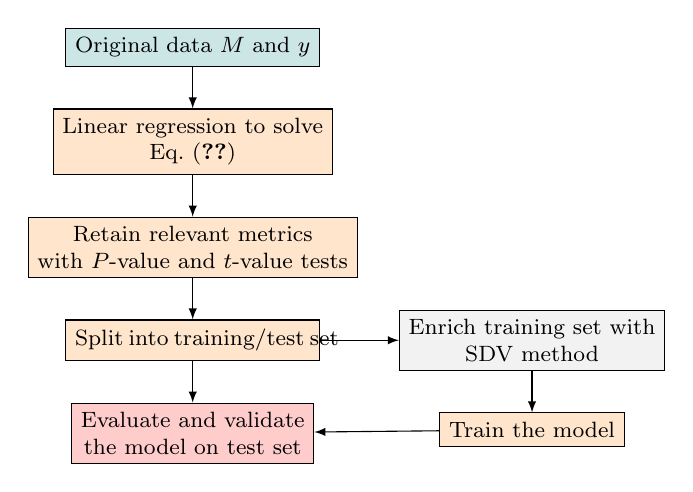
\begin{tikzpicture}
        \tikzstyle{block} = [%
        draw, fill=blue!20, align=center, rectangle, font=\footnotesize,
        execute at begin node={\begin{varwidth}{10em}},
        execute at end node={\end{varwidth}}]
        
        \node[block, fill=teal!20] (A) at (4,0){Original data $M$ and $y$};
        \node[block, fill=orange!20, below=1.5em of A] (B){Linear regression to solve \\ Eq.~\eqref{normal_linear_regresion}};
    	\node[block, fill=orange!20, below=1.5em of B] (C){Retain relevant metrics \\with $P$-value and $t$-value tests};
    	\node[block, fill=orange!20, below=1.5em of C] (D) {Split into training/test set};
    	\node[block, fill=gray!10, right=of D] (E) {Enrich training set with\\SDV method};
    	\node[block, fill=orange!20, below=1.5em of E] (F) {Train the model};
    	\node[block, fill=red!20, below=1.5em of D] (G) {Evaluate and validate\\the model on test set};
        
    	\draw[-latex] (A) -- (B);
            \draw[-latex] (B) -- (C);
    	\draw[-latex] (C) -- (D);
    	\draw[-latex] (D) -- (E);
        \draw[-latex] (E) -- (F);% node[pos=0.5, right] {$y_{\text{training}}$};
        \draw[-latex] (F) -- (G);% node[pos=0.5, below] {$\theta^*$};
        \draw[-latex] (D) -- (G);% node[pos=0.5, right] {$y_{\text{test}}$};
    \end{tikzpicture}
    \caption{\footnotesize Flowchart of the model training and testing process.}
    \label{flow_diagram}
 \end{figure}



% \begin{figure}[t]
%   \centering
%     \includegraphics[width=0.49\linewidth]{Images/explained_variance_c_rap.png}
%     \includegraphics[width=0.49\linewidth]{Images/loadings_c_rap.png}
%   \caption{\footnotesize On the left,  the explained variance of matrix $M$. On the right, the contribution of each metric to each principal component is represented by the normalized linear combination coefficients.}
%   \label{explained_variance}
% \end{figure}

\subsubsection{Synthetic data vault}
In current practices, the data are usually divided into training and validation sets using a ratio of 75\% to 25\%.
%as described in \cite{chollet2021deep}. 
By removing the columns $s_{\mathcal{G}}$ and $c_{\mathcal{G}}$, and selecting 10 random samples each for safety and comfort training, the matrix $M \in \mathbb{R}^{20 \times 4}$, the vector $\theta \in \mathbb{R}_{>0}^4$ in Eq.~\eqref{lineal_form} and the original data $y \in \mathbb{R}^{4}$ in Eq.~\eqref{approach_function} are redefined according to the $10$ selected samples. With the remaining 4 samples used for validation. 

% To enhance the conditioning of matrices for the 10-samples chosen for training by increasing the data size, we employ the Synthetic Data Vault (SDV) method for creating synthetic data\cite{7796926}. The generation is based on the original data distribution, ensuring that the two datasets maintain similar statistical characteristics. By Lemma.~\ref{lema_nnls}, the linear regression can be treated with non-negative least squares (NNLS), which is well referenced in \cite{lawson1995solving}. Refer to the Fig.~\ref{flow_diagram} for a breakdown of the complete process. 

To improve matrix conditioning for the 10 training samples, we use the Synthetic Data Vault (SDV) method to generate synthetic data \cite{7796926}. The synthetic data maintains the original distribution, ensuring similar statistical properties. By Lemma \ref{lema_nnls}, linear regression is treated with non-negative least squares (NNLS), as detailed in \cite{lawson1995solving}. See Fig.~\ref{flow_diagram} for the process breakdown.


%-----------------------------
\begin{lemma}
\label{lema_nnls}
After selecting significant metrics and enriching the training data using the SDV method, solving Problem~$1$ under the linear model structure is equivalent to find the optimal $\tilde{\theta}$:
\begin{align}
        \label{min_nnlss}
        &  \tilde{\theta} = \underset{\hat{\theta} \in \mathbb{R}_{\geq 0}^4}{\operatorname{argmin}}  \left\|  M \hat{\theta} - y \right\|^2  = \underset{\hat{\theta} \in \mathbb{R}^4}{\operatorname{argmin}}  \left\|  M \hat{\theta} - y \right\|^2. 
   \end{align}
\end{lemma}
%
\begin{proof} This equivalence can be easily demonstrated by noting that the only selected metric inherently exhibits non-decreasing monotonic behavior with respect to their CSCS values. Provided that all components of the $\theta$ parameter vector are positive semidefinite, then the linear regression structure inherits non-decreasing monotonic properties of the metrics. 
\end{proof}
%-------------------------------

\subsection{Comparison between the linear regression and  Ensemble ML-based models}


We employ NNLS using only $l_{\mathcal{G}}$, as it is the only metric shown to significantly predict perceived safety and comfort, as indicated in Table \ref{p_value_safety_comfort}. The resulting coefficients are as follows: 
\begin{equation}
\label{nnls_results_cv}
    \tilde{\theta} = \left [ 0.41, 0.58,  0.45, 0.57  \right ]^{T}.
\end{equation}
% Since $l_{\mathcal{G}}$ is the metric most strongly correlated with perceived safety and comfort, we validate the reliability of our linear approach in addressing Problem~$1$ by comparing its results with those obtained using the AutoGluon Auto-ML ensemble method \cite{erickson2020autogluon}. }Auto-ML ensemble methods combine various individual models, such as trees, neural networks, support vector machines, and regression models, to enhance overall prediction accuracy and robustness. 

% Fig.~\ref{safety_comfort_prediction_CV} illustrates the outcomes of both approaches, NNLS and Auto-ML ensemble, where we observe that both approaches provide similar results, and both effectively capture significant aspects of perceived safety and comfort. Therefore, we choose to adopt NNLS as our definitive model for predicting safety and comfort due to its acceptable results and simplicity.
Since $l_{\mathcal{G}}$ is the most correlated metric with perceived safety and comfort, we validate our linear approach by comparing its results with those from the AutoGluon Auto-ML ensemble method \cite{erickson2020autogluon}. Auto-ML combines models like trees, neural networks, and regression to improve prediction accuracy.

Fig.~\ref{safety_comfort_prediction_CV} shows that both NNLS and Auto-ML ensemble yield similar results, effectively capturing key aspects of safety and comfort. Therefore, we select NNLS for its simplicity and acceptable performance.




\begin{figure*}[t]
\vspace{0.2cm}
  \centering
 \includegraphics[width=0.49\linewidth]{Images/safety_prediction.png}
  \includegraphics[width=0.49\linewidth]{Images/comfort_prediction.png}
  \caption{\footnotesize Predicted values versus the actual values of perceived safety (right) and comfort (left). The average error is $2.23$ \% and $3.15$ \% for Auto-ML Ensemble and NNLS, respectively, for safety, and $5.99$ \% and $7.36$ \% for Auto-ML Ensemble and NNLS, respectively, for comfort.}
  \label{safety_comfort_prediction_CV}
\end{figure*}


\section{Network optimal design}
\label{optimization_problem}


%\subsection{Problem formulation}
% In this section, we use the previously identified linear regression model to formulate our network-upgrade optimization problem. Each upgrade of the cycling infrastructure (i.e., increasing the CSCS value of a road segment or edge) incurs a cost per meter. The CSCS values can transition from any value in $\mathcal{K}$ to any equal or greater value in $\mathcal{K}$, with the requirement that these upgrades remain discrete. Our objective is to optimize the selection of edges to be upgraded in order to maximize the expected perceived safety and comfort of a specific cycling network $\mathcal{G}$ within a fixed budget $B$. We introduce the following notations:
In this section, we formulate the network-upgrade optimization problem using the identified linear regression model. Upgrading a road segment increases its CSCS value and incurs a cost per meter. CSCS values can only increase within the set $\mathcal{K}$ in discrete steps. The goal is to select edges for upgrade to maximize expected perceived safety and comfort in a cycling network $\mathcal{G}$, while staying within a fixed budget $B$. We introduce the following notations:

\begin{itemize}
    \item $\omega_{0} = \left [ \omega_{1}, \ldots, \omega_{e}, \ldots, \omega_{|E|} \right ]$ are the original edge weights (CSCS) of the graph $\mathcal{G}$ to be optimized.
    \item $\tilde \omega = \left [ \tilde{\omega}_{1},  \ldots, \tilde{\omega}_{e}, \ldots,\tilde{\omega}_{|E|} \right ] \in \Omega $ are the candidate weights to be optimized, with,
    \begin{equation} \nonumber
        \Omega = \left \{ \tilde{\omega} \in \mathbb{N}^{|E|} \colon \omega_{e} \leq \tilde{\omega}_{e} \leq \omega_{\text{DoS}_6},  \forall e \in \left \{1,2, \ldots, |E| \right \}  \right\}.
    \end{equation} 
\end{itemize}
Based on the linear model structure derived above and the identified parameters, we can now define two predicted model outputs, each with different CSCS weights,
\begin{equation*}
 \hat{y}_{\omega_{0}} = M_{\omega_{0}} \tilde{\theta}, \quad \quad \hat{y}(\tilde{\omega}) = M_{\tilde{\omega}}\tilde{\theta}
\end{equation*}
with $\theta^{\ast}$ as defined in Eq.~\eqref{nnls_results_cv}.  $M_{\omega_{0}} \in~\mathbb{R}^{2 \times 4}$, and $M_{\tilde{\omega}} \in~\mathbb{R}^{2 \times 4}$ are matrices following similar structure as $M$, with the $s_{\mathcal{G}}$ and $c_{\mathcal{G}}$ columns removed (as suggested by p-value test in previous section). They are defined as:
\begin{equation} \nonumber
    M_{\omega_{0}} = 
    \begin{bmatrix}
        m_{\omega_{0}} & 0\\ 
        0 & m_{\omega_{0}}
            \end{bmatrix} , \quad \quad 
        M_{\tilde{\omega}} = \begin{bmatrix}
        m_{\tilde{\omega}} & 0\\ 
        0 & m_{\tilde{\omega}}
    \end{bmatrix}
\end{equation}
with $m_{\omega_{0}}$ and $m_{\tilde{\omega}}$ in $\mathbb{R}^{1 \times 2}$, 
$$
m_{\omega_{0}} = \left[   1,  l_{\mathcal{G}} \right ],  \quad \quad m_{\tilde{\omega}} = \left[   1,  l_{\mathcal{G}_{\tilde{\omega}}} \right ]
$$
where $l_{\mathcal{G}_{\tilde{\omega}}}$ is computed in $\mathcal{G}$ with the CSCS changed  to  $\tilde{\omega}$. Denoting $\pi(\omega_{e},\tilde{\omega}_{e})$ the cost or price per meter of upgrading edge $e$ from $\omega_{e}$ to $\tilde{\omega}_{e}$, the optimization problem can now be formulated as follows:

\begin{problem}[Network-upgrade optimization problem]
    \begin{align}
        \label{problem_a_1}
        \omega^{\ast} &= \; \underset{\tilde{\omega} \in \Omega}{\operatorname{argmax}} \; ||\hat{y}_{\omega_{0}}- \hat{y}(\tilde{\omega}) || \\
        &= \label{problem_a_2} \; \underset{\tilde{\omega} \in \Omega}{\operatorname{argmax}} \; ||(M_{\omega_{0}}- M_{\tilde{\omega}}) \tilde{\theta} || \\
        & \label{problem_a_3} \text{under} \quad   \sum_{e=1}^{|E|} d_{e} \cdot \pi(\omega_{e},\tilde{\omega}_{e}) \leq B,
    \end{align}
\end{problem}
%
% Problem~$2$ is NP-hard and finding the optimal solution has a computational complexity of $\mathcal{O}(6^{|E|})$ (details given in Appendix~A). The objective function and constraints are nonlinear and relate to the Knapsack problem, hence in preliminary studies we tried some off-the-shelf solvers  for a real cycling network Section~\ref{Grenoble_case}. However, we found that for large-scale networks they tend to be really slow and do not converge even slightly to the optimal. As a consequence, we chose to develop our own dedicated algorithm to approximate the solution that we named the MLCC (Maximize Largest Connected Component) algorithm. This algorithm has complexity of $\mathcal{O}(|E||V|^{4})$. Its solution will still be denoted as $\omega^{\ast}$ for the sake of simplicity.
Problem~$2$ is NP-hard, with an optimal solution complexity of $\mathcal{O}(6^{|E|})$ (see Appendix~A). The objective function and constraints are nonlinear and related to the Knapsack problem. Preliminary tests with off-the-shelf solvers on real cycling networks (Section~\ref{Grenoble_case}) showed that they were too slow and failed to converge for large networks. To address this, we developed the MLCC (Maximize Largest Connected Component) algorithm, which approximates the solution with a reduced complexity of $\mathcal{O}(|E||V|^{4})$. For simplicity, its solution is still denoted as $\omega^{\ast}$.





\subsection{MLCC algorithm} 
\label{section:mlcc}

The concept is to systematically update edges, prioritizing the expansion of sub-networks featuring the largest connected component with the highest CSCS. The rationality for this choice is the observation in Section~\ref{linear_regression_model} that $l_{\mathcal{G}}$ is the only metric significantly affecting the prediction of perceived safety and comfort.

Hereafter, we call shortest CSCS path the shortest path when the basis is the geographical inverted weights $d_e~\cdot ~\omega_{\text{DoS}_{(7-\text{DoS}(e))}}$, where $\text{DoS}(e)$ as in Section~\ref{closenness_metric}. At every step of the algorithm, upgrades are done according to the budget constraints. If the budget is fully used then the algorithm ends. The output is a list with the upgrades of the CSCS for each edge in $E$.
The proposed algorithm is described below, the detailed flowchart can be found in Appendix~B.

For every connected component, do:
\begin{itemize}
     \item[1)] \textit{Obtain a single connected component with maximum CSCS:}  Identify the largest connected component of edges with the highest CSCS. 
     \begin{itemize}
         \item[1.1)] If CSCS~$< \omega_{\text{DoS}_6}$, then upgrade it to $\omega_{\text{DoS}_6}$;
         \item[1.2)] Otherwise, if there are several connected components of $\omega_{\text{DoS}_6}$: start connecting them from largest to smallest by upgrading the connecting edges to the $\omega_{\text{DoS}_6}$ score using shortest CSCS path. 
     \end{itemize}
     
     We obtain one single connected sub-network with scores $\omega_{\text{DoS}_6}$ referred to as $\widehat{C}$.
     
    \item[2)] \textit{Enlarge $\widehat{C}$ with lower CSCS connected components:} Denote $C_{\tilde{\gamma}}$ the largest connected component with highest score $\tilde{\gamma}< \omega_{\text{DoS}_6}$.
    Find the shortest CSCS path between $\widehat{C}$ and $C_{\tilde{\gamma}}$, and upgrade the edges along this path. Then upgrade edges of $C_{\tilde{\gamma}}$ to the $\omega_{\text{DoS}_6}$. This process progressively enlarges $\widehat{C}$ at each step. Iterate this step by considering the next largest connected component  $C_{\tilde{\gamma}}$ with the highest $\tilde{\gamma}<\omega_{\text{DoS}_6}$. This iterative process continues until the budget is fully utilized or all edges are upgraded to their maximum CSCS level. 
    
\end{itemize}
 


\begin{figure}[t]
\vspace{0.2cm}
  \centering
  \captionsetup[subfigure]{font={footnotesize}, labelfont={footnotesize, bf}, textfont={footnotesize, rm}}

  \subfloat[Benchmark example]{\includegraphics[width=0.55\linewidth]{Images/Plot_ITS_academic_example_original.png}\label{ae_1}}
  % \hspace{0.001\linewidth} % Adjust horizontal space as needed
  \subfloat[Optimal]{\includegraphics[width=0.40\linewidth]{Images/Plot_T_ITS_academic_example_optimal.png}\label{ae_2}} \\
  \vspace{0.02\linewidth} % Adjust horizontal space as needed
  \subfloat[MLCC]{\includegraphics[width=0.40\linewidth]{Images/Plot_T_ITS_academic_example_mlcc.png}\label{ae_5}}
  \hspace{0.03\linewidth} % Adjust vertical space as needed
  \subfloat[SGA]{\includegraphics[width=0.40\linewidth]{Images/Plot_T_ITS_academic_example_sga.png}\label{ae_3}}\\
  \vspace{0.02\linewidth} % Adjust horizontal space as needed
  \subfloat[SGA-MLCC]{\includegraphics[width=0.40\linewidth]{Images/Plot_T_ITS_academic_example_sga_mlcc.png}\label{ae_4}}
  \hspace{0.03\linewidth} % Adjust horizontal space as needed
  \subfloat[Bayesian]{\includegraphics[width=0.40\linewidth]{Images/Plot_T_ITS_academic_example_bayesian.png}\label{ae_6}}
  
  \caption{\footnotesize(a) Original configuration, (b) optimal solution configuration, (c) MLCC algorithm configuration, (d) SGA configuration, (e) SGA-MLCC configuration and (f) Bayesian algorithm configuration: These configurations aim to enhance perceived safety with $i = 7$, corresponding to $\alpha_7 \approx 0.35\%$ of the total budget required for a full network upgrade ($B_{\text{max}}=$22,010€).}
  \label{academic_example}
\end{figure}

% \begin{table*}[t]
% \centering
% \begin{tabular}{|c|c|c|c|c|c|c|c|c|}
% \hline
% \textbf{Algorithm} & \multicolumn{4}{|c|}{\textbf{Safety}} & \multicolumn{4}{|c|}{\textbf{Comfort}} \\ \hline
%  & $\alpha = \frac{1}{4}$ & $\alpha = \frac{1}{2}$ & $\alpha = \frac{3}{4}$ & $\alpha = 1$ & $\alpha = \frac{1}{4}$ & $\alpha = \frac{1}{2}$ & $\alpha = \frac{3}{4}$ & $\alpha = 1$ \\ \hline
% Optimal & 44.52 s & 2.47 m & 3.06 m & 3.40 m & 44.52 s & 5.10 m & 6.21 m & 7.11 m \\ \hline
% MLLC & 0.011 s & 0.012 s & 0.011 s & 0.011 s & 0.011 s & 0.011 s & 0.011 s & 0.012 s \\ \hline
% SGA & 21.89 s & 25.09 s & 28.97 s & 27.90 s & 25.23 s & 9.58 s & 27.02 s & 28.63 s \\ \hline
% SGA-MLCC & 12.62 & 15.56 s & 28.65 s & 27.55 s & 12.49 s & 9.18 s & 13.21 s & 12.72 s \\ \hline
% Bayesian & 1.53 m & 1.14 m & 1.45 m & 2.03 m & 1.74 m & 1.67 m & 1.94 m & 1.56 m \\ \hline
% \end{tabular}
% \caption{Computational time of bechmark example}
% \label{bench_mark_time_table}
% \end{table*}


%%%%%%%%%%%%%%%%%%%%%%%%%%%%%%%%%%%%%%%%%%%%
%%%%%%%%%%%%%%%%%%%%%%%%%%%%%%%%%%%%%%%%%%%%
\begin{figure*}[h!]
\vspace{0.2cm}
  \centering
  \captionsetup[subfigure]{font={footnotesize}, labelfont={footnotesize, bf}, textfont={footnotesize, rm}}

    \subfloat[]{\includegraphics[width=0.95\linewidth]{Images/maximize_safety_academic_example_LCC.png}\label{ae_1_r}}
  \hspace{0.03\linewidth} % Adjust horizontal space as needed
  \subfloat[]{\includegraphics[width=0.42\linewidth]{Images/AE_comparation_GA_LCC_safety.png}\label{ae_2_r}}
  \hspace{0.03\linewidth} % Adjust horizontal space as needed
  % \subfloat[]{\includegraphics[width=0.43\linewidth]{Images/AE_comparation_GA_LCC_safety_time.png}\label{ae_4_r}} 
  % \vspace{0.2cm}
  % \subfloat[]{\includegraphics[width=0.35\linewidth]{Images/AE_comparation_GA_LCC_comfort.png}\label{ae_3_r}}
  \subfloat[]{\includegraphics[width=0.40\linewidth]{Images/Grenoble_comparation_GA_LCC_safety_legend.png}\label{ae_legend}}
  % \vspace{0.2cm} % Adjust vertical space as needed

  
  % \hspace{0.03\linewidth} % Adjust horizontal space as needed
  % \subfloat[]{\includegraphics[width=0.35\linewidth]{Images/AE_comparation_GA_LCC_comfort_time.png}\label{ae_5_r}}
  % \subfloat[]{\includegraphics[width=0.19\linewidth]{Images/AE_comparation_GA_LCC_safety_time_legend.png}\label{ae_legend_time}}

  \caption{\footnotesize (a) Results of solving Problem~$2$ using the optimal, MLCC, SGA, SGA-MLCC, and Bayesian algorithms on the benchmark network. The percentage improvement is calculated as \% = $|\hat{y}_{\omega_{0}} - \hat{y}(\omega^{\ast})| \times 100 / |\hat{y}_{FS} - \hat{y}_{\omega_0}|$. (b) Performance evolution of the SGA and SGA-MLCC algorithms over generations for safety with (c) providing the legend. $B_{\max}=$  22, 010 €.} 
\label{ae_algorithms_comparation}
  % Table inside figure environment
  \vspace{10pt} % Add vertical space between the figure and the table

  \begin{minipage}{\textwidth}
    \centering
    \captionsetup{labelformat=empty} % Temporarily empty label format
    \renewcommand{\thetable}{TABLE \arabic{table}} % Change table numbering
    \footnotesize
    \begin{tabular}{|c|c|c|c|c|c|c|c|c|c|c|}
    \hline
    \textbf{Algorithm} & \multicolumn{10}{|c|}{\textbf{Time}} \\ \hline
     & $i = 0$ & $i = 1$ & $i = 2$ & $i = 3$ & $i = 4$ & $i = 5$ & $i = 6$ & $i = 7$ & $i = 8$ & $i = 9$ \\ \hline
    Optimal & 4.96 s & 4.33 s & 4.35 s & 4.46 s & 6.0 s & 11.19 s & 32.62 s & 1.63 m & 3.04 m & 4.7 m \\ \hline
 MLCC & 0.014 s & 0.011 s & 0.011 s & 0.011 s & 0.011 s & 0.011 s & 0.011 s & 0.014 s & 0.012 s & 0.011 s \\ \hline
SGA & 6.7 s & 6.99 s & 7.28 s & 8.39 s & 8.46 s & 8.72 s & 7.58 s & 8.91 s & 9.89 s & 10.6 s \\ \hline
SGA-MLCC & 7.8 s & 8.2 s & 8.35 s & 8.6 s & 7.45 s & 7.69 s & 9.18 s & 9.22 s & 10.16 s & 10.82 s \\ \hline
Bayesian & 1.35 m & 1.45 m & 1.45 m & 1.63 m & 1.88 m & 1.98 m & 1.96 m & 1.89 m & 1.96 m & 2.03 m \\ \hline
%  & \multicolumn{10}{|c|}{\textbf{Comfort}} \\ \hline
%     Optimal & 4.31 s & 4.44 s & 4.43 s & 4.87 s & 6.25 s & 11.24 s & 32.73 s & 1.61 m & 2.98 m & 4.65 m \\ \hline
%  MLCC & 0.011 s & 0.012 s & 0.012 s & 0.011 s & 0.014 s & 0.014 s & 0.014 s & 0.015 s & 0.012 s & 0.011 s \\ \hline
% SGA & 18.37 s & 18.48 s & 18.48 s & 18.02 s & 16.87 s & 18.08 s & 21.21 s & 18.46 s & 20.06 s & 22.01 s \\ \hline
% SGA-MLCC & 7.36 s & 16.67 s & 19.34 s & 20.23 s & 10.52 s & 17.43 s & 18.69 s & 20.74 s & 14.38 s & 9.8 s \\ \hline
% Bayesian & 1.47 m & 1.42 m & 1.67 m & 1.48 m & 1.95 m & 1.56 m & 1.98 m & 2.0 m & 2.03 m & 2.06 m \\ \hline
    \end{tabular}
    \caption{TABLE V: Calculation time for the benchmark example}
    \label{bench_mark_time_table}
  \end{minipage}
\end{figure*}
\newpage
%%%%%%%%%%%%%%%%%%%%%%%%%%%%%%%%%%%%%%%%%%%%
%%%%%%%%%%%%%%%%%%%%%%%%%%%%%%%%%%%%%%%%%%%%

\section{Benchmark  example}
\label{academic_example_section}



% \begin{figure*}[t]
%   \centering
%   \captionsetup[subfigure]{font={footnotesize}, labelfont={footnotesize, bf}, textfont={footnotesize, rm}}

%   \subfloat[]{\includegraphics[width=0.95\linewidth]{Images/maximize_safety_academic_example_LCC.png}\label{ae_1_r}}
%   \hspace{0.03\linewidth} % Adjust horizontal space as needed
%   \subfloat[]{\includegraphics[width=0.35\linewidth]{Images/AE_comparation_GA_LCC_safety.png}\label{ae_2_r}}
%   \hspace{0.03\linewidth} % Adjust horizontal space as needed
%   \subfloat[]{\includegraphics[width=0.35\linewidth]{Images/AE_comparation_GA_LCC_comfort.png}\label{ae_3_r}}
%   \subfloat[]{\includegraphics[width=0.23\linewidth]{Images/AE_comparation_GA_LCC_safety_legend.png}\label{ae_legend}}
%   % \vspace{0.2cm} % Adjust vertical space as needed

%   \subfloat[]{\includegraphics[width=0.35\linewidth]{Images/AE_comparation_GA_LCC_safety_time.png}\label{ae_4_r}}
%   \hspace{0.03\linewidth} % Adjust horizontal space as needed
%   \subfloat[]{\includegraphics[width=0.35\linewidth]{Images/AE_comparation_GA_LCC_comfort_time.png}\label{ae_5_r}}
%   \subfloat[]{\includegraphics[width=0.23\linewidth]{Images/AE_comparation_GA_LCC_safety_time_legend.png}\label{ae_legend_time}}

%   \caption{\footnotesize (a) Result of solving Problem~$2$ by the optimal, MLCC, SGA, SGA-MLCC and Bayesian algorithms in the benchmark example. \% = $|\hat{y}_{\omega_{0}}- \hat{y}(\omega^{\ast})| \times 100/|\hat{y}_{FS}-\hat{y}_{\omega_0}|$. (b) and (c) show the evolution of the SGA and SGA-MLCC algorithms for safety and comfort, respectively. (e) and (f) show the cumulative time of the SGA and SGA-MLCC through the generations.}
%   \label{ae_algorithms_comparation}
% \end{figure*}

% \begin{table*}[t]
% \centering
% \begin{tabular}{|c|c|c|c|c|c|c|c|c|}
% \hline
% \textbf{Algorithm} & \multicolumn{4}{|c|}{\textbf{Safety}} & \multicolumn{4}{|c|}{\textbf{Comfort}} \\ \hline
%  & $\alpha = \frac{1}{4}$ & $\alpha = \frac{1}{2}$ & $\alpha = \frac{3}{4}$ & $\alpha = 1$ & $\alpha = \frac{1}{4}$ & $\alpha = \frac{1}{2}$ & $\alpha = \frac{3}{4}$ & $\alpha = 1$ \\ \hline
% Optimal & 44.52 s & 2.47 m & 3.06 m & 3.40 m & 44.52 s & 5.10 m & 6.21 m & 7.11 m \\ \hline
% MLLC & 0.011 s & 0.012 s & 0.011 s & 0.011 s & 0.011 s & 0.011 s & 0.011 s & 0.012 s \\ \hline
% SGA & 21.89 s & 25.09 s & 28.97 s & 27.90 s & 25.23 s & 9.58 s & 27.02 s & 28.63 s \\ \hline
% SGA-MLCC & 12.62 s & 15.56 s & 28.65 s & 27.55 s & 12.49 s & 9.18 s & 13.21 s & 12.72 s \\ \hline
% Bayesian & 1.53 m & 1.14 m & 1.45 m & 2.03 m & 1.74 m & 1.67 m & 1.94 m & 1.56 m \\ \hline
% \end{tabular}
% \caption{Computational time of benchmark example}
% \label{bench_mark_time_table}
% \end{table*}






% \begin{figure}[t]
%   \centering

%   % First figure with label to the right
%   \begin{minipage}[t]{0.8\linewidth}
%     \centering
%     \includegraphics[width=\linewidth]{Images/maximize_safety_academic_example_LCC.png}
%   \end{minipage}%
%   \begin{minipage}[t]{0.2\linewidth}
%     \centering
%     \raisebox{6.0\height}{(a)}
%   \end{minipage}

%   \vspace{0.2cm} % Adjust vertical space as needed

%   % Second figure with label to the right
%   \begin{minipage}[t]{0.8\linewidth}
%     \centering
%     \includegraphics[width=\linewidth]{Images/AE_comparation_GA_LCC_safety.png}
%   \end{minipage}%
%   \begin{minipage}[t]{0.2\linewidth}
%     \centering
%     \raisebox{6.0\height}{(b)}
%   \end{minipage}

%   \vspace{0.2cm} % Adjust vertical space as needed

%   % Third figure with label to the right
%   \begin{minipage}[t]{0.8\linewidth}
%     \centering
%     \includegraphics[width=\linewidth]{Images/AE_comparation_GA_LCC_comfort.png}
%   \end{minipage}%
%   \begin{minipage}[t]{0.2\linewidth}
%     \centering
%     \raisebox{6.0\height}{(c)}
%   \end{minipage}

%    % Third figure with label to the right
%   \begin{minipage}[t]{0.8\linewidth}
%     \centering
%     \includegraphics[width=\linewidth]{Images/AE_comparation_GA_LCC_safety_time.png}
%   \end{minipage}%
%   \begin{minipage}[t]{0.2\linewidth}
%     \centering
%     \raisebox{6.0\height}{(d)}
%   \end{minipage}

%   % Third figure with label to the right
%   \begin{minipage}[t]{0.8\linewidth}
%     \centering
%     \includegraphics[width=\linewidth]{Images/AE_comparation_GA_LCC_comfort_time.png}
%   \end{minipage}%
%   \begin{minipage}[t]{0.2\linewidth}
%     \centering
%     \raisebox{6.0\height}{(e)}
%   \end{minipage}

%   \caption{\footnotesize (a) Result of solving Problem~$2$ by the optimal, MLCC, SGA, SGA-MLCC and Bayesian algorithms in the benchmark example. \% = $|\hat{y}_{\omega_{0}}- \hat{y}(\omega^{\ast})| \times 100/|\hat{y}_{FS}-\hat{y}_{\omega_0}|$. (b) and (c) show the evolution of the SGA and SGA-MLCC algorithms for safety and comfort, respectively.}
%   \label{ae_algorithms_comparation}
% \end{figure}
Our goal now is to compare the performance of our MLCC algorithm, developed to tackle Problem~$2$, against a straightforward benchmark example where the optimal solution is determined by exhaustively evaluating all possible combinations. Additionally, we will compare it with three solvers to measure the distances to optimality.

Let $B = \alpha \cdot B_{\text{max}}$, be the available budget for optimization, with $B_{\text{max}}$ being the budget required to reach the FS graph (with corresponding prediction $\hat y_{FS}$), and $\alpha \in \left [ 0,1\right]$. The cost per meter to upgrade the infrastructure along an edge is set to reflect different construction costs between levels, following Cerema's cost \cite{cerema2024_cost} studies. 

We select 10 logarithmically spaced values of $\alpha$ between 0.01 and 1 to examine the behavior of our analysis near zero.
\begin{equation}
\alpha_i = 10^{\left(a + i \cdot \frac{b - a}{9}\right)}, \quad i \in \{0, 1, \dots, 9\},    
\end{equation}
where
\begin{equation}
    a = \log_{10}(0.01), \quad b = \log_{10}(1).
\end{equation}

In Fig.~\ref{ae_1}, we display our benchmark example consisting of 10 nodes and 11 edges. Figure \ref{academic_example} (b)-(f) compare the configurations derived from: (1) the optimal solution obtained by evaluating all 138,240 possible combinations via brute force, (2) our MLCC algorithm, (3) a standard genetic algorithm (SGA) \cite{pygmo}, (4) the SGA initialized with the output of the MLCC algorithm (SGA-MLCC), and (5) a Bayesian optimization package in Python \cite{bayesian_2014}, all designed to approximate the optimal solution within a reasonable time frame. These comparisons are made to approximate the optimal solution for safety using approximately one third of the budget ($\alpha_{7} \approx 0.35$). While our MLCC algorithm does not precisely reproduce the optimal solution, it exhibits strong similarities with all other algorithms. Notably, all solutions prioritize maximizing the connectivity of $\omega_{\text{DoS}_6}$ score segments rather than upgrading isolated links. This is because enhancing a single, unconnected segment to a high $\omega_{\text{DoS}_6}$ scores would inefficiently allocate the budget without significantly improving perceived safety and comfort across the network,  demonstrating the MLCC algorithm's strong performance in delivering a practical and computationally efficient solution for larger networks, while acknowledging that the exact optimality gap remains uncertain.
%While our MLCC algorithm does not exactly reproduce the optimal solution, it shows remarkable similarities with all other algorithms. For example, all solutions attempt to maximize the largest connected component of score $\omega_{\text{DoS}_6}$
In Fig.~\ref{ae_algorithms_comparation}a, we illustrate the improvements in normalized perceived safety and comfort across four different values of $\alpha$. At $\alpha_{7}$, both the optimal solution and the Bayesian algorithm achieve approximately a 29\% improvement in perceived safety and comfort, whereas our algorithm achieves around 26\%. Although our algorithm does not reach the optimal level, it provides a favorable outcome. 

Fig.~\ref{ae_algorithms_comparation}b shows the evolution of SGA and SGA-MLCC over 80 generations, respectively. This figure demonstrates that, in most cases, SGA-MLCC approaches the optimal solution more closely than the standard SGA. This suggests that using the MLCC results as the initial population for the SGA is a beneficial strategy. Finally, Table V presents the computation times, showing that the MLCC operates significantly faster, making it especially beneficial for large-scale, real-world cycling networks.

\section{Sioux Falls and Grenoble Cycling Network}
\label{Grenoble_case}

% To demonstrate a well-known example in transportation research, we use the Sioux Falls network, which consists of 24 nodes and 38 edges with randomly assigned DoS values, as shown in Fig.~\ref{sioux_falls_network}. However, as network size and complexity increase, finding an optimal solution becomes computationally infeasible due to the exponential growth in the number of possible configurations. For example, while evaluating a single configuration for the Sioux Falls network takes approximately 0.009 seconds, evaluating all possible combinations would require more than a trillion years. This highlights the need for efficient algorithms like MLCC to handle such large-scale problems. 

% The results of our analysis are presented in Appendix~C, where we show that MLCC performs competitively compared to other algorithms. Importantly, the SGA-MLCC approach consistently achieves superior performance, in line with observations from the academic example, where SGA-MLCC closely approximated the optimal solution. Building on these findings, and now that this widely recognized benchmark has been tested, we plan to extend our analysis to a real-world cycling network, such as the Grenoble cycling network.

% To illustrate a well-known transportation research example, we use the Sioux Falls network (24 nodes, 38 edges) with randomly assigned DoS values (Fig.~\ref{sioux_falls_network}). As network size grows, computing an optimal solution becomes infeasible due to exponential complexity. For instance, while evaluating one configuration takes 0.009 seconds, testing all possibilities would take over a trillion years, underscoring the need for efficient algorithms like MLCC. Appendix~C presents our analysis, showing MLCC's competitive performance. Notably, SGA-MLCC consistently performs best, aligning with prior findings where it closely approximated the optimal solution. With this benchmark validated, we now extend our analysis to a real-world case: the Grenoble cycling network.  

% In Fig.~\ref{maximize_three_algorithms_grenoble}a it is presented the comparison of algorithms for the Grenoble cycling network, showing that the MLCC algorithm consistently outperforms the others. Fig.~\ref{maximize_three_algorithms_grenoble}b shows the performance evolution of the SGA and SGA-MLCC algorithms over 80 generations. The SGA-MLCC algorithm fails to outperform MLCC, ultimately converging to the same solution. Despite parameter adjustments and variations in the initial population, MLCC consistently yields the best results. Table~IV shows computing times for all algorithms, demonstrating that MLCC not only achieves the best performance but also operates faster. This highlights its robustness and efficiency in solving large network problems, making it the preferred choice over heuristic methods. Fig.~\ref{grenoble_changes} depicts the upgraded Grenoble cycling network using MLCC with $\alpha_7$. Thus, MLCC is used to approximate the global optimum across 14 French cities.




To illustrate a well-known transportation research example, we use the Sioux Falls network (24 nodes, 38 edges) \cite{chakirov2016sioux} with randomly assigned DoS values 
(Fig.~\ref{sioux_falls_network}). 
\begin{figure}[H]
    \centering
    \includegraphics[width=0.42\textwidth]{Images/Sioux_Falls.png}
    \caption{\footnotesize Sioux Falls cycling network}
    \label{sioux_falls_network}
\end{figure}

\begin{figure}[H]
    \centering
\includegraphics[width=\columnwidth]{Images/Map_and_scale_changes.pdf}
    \caption{\footnotesize Cycling network of Grenoble, France, after being upgraded using MLCC with $\alpha_7 \approx 0.35$.}
    \label{grenoble_changes}
\end{figure}
As network size grows, computing an optimal solution becomes infeasible due to exponential complexity. For example, evaluating one configuration takes 0.009 seconds, but testing all possibilities would take over a trillion years, highlighting the need for efficient algorithms like MLCC. Appendix~C shows that MLCC performs competitively, with SGA-MLCC consistently achieving the best results. Our benchmark analysis in the previous section suggests that the algorithm is relatively close to the optimal solution, and after validating it on the well-known Sioux-Falls benchmark, we now extend our approach to a real case: the Grenoble cycling network.

%, closely approximating the optimal solution. With this benchmark validated, we now apply our analysis to a real-world case: the Grenoble cycling network.  

Fig.~\ref{maximize_three_algorithms_grenoble}a compares algorithm performance for the Grenoble network, showing that MLCC consistently outperforms others. Fig.~\ref{maximize_three_algorithms_grenoble}b tracks SGA and SGA-MLCC performance over 80 generations, revealing that SGA-MLCC fails to surpass MLCC and ultimately converges to the same solution. Despite parameter adjustments and initial population variations, MLCC consistently yields the best performance. Table~IV further demonstrates MLCC’s advantage, achieving the best results with significantly lower computation time. This underscores its efficiency in solving large network problems, making it the preferred choice over heuristic methods. Fig.~\ref{grenoble_changes} visualizes the upgraded Grenoble cycling network using MLCC with $\alpha_7$. Extending this approach, MLCC is applied to optimize cycling networks across 14 French cities.  


% Appendix~C shows that MLCC performs competitively, with SGA-MLCC consistently achieving superior results, closely approximating the optimal solution.
% Unfortunately, meanwhile the amount of edges and nodes increase the optimal is not possible compute anymore, for example well-known transportation example as the Sioux Falls network (24 nodes, 38 edges) with randomly assigned DoS values (Fig.~\ref{sioux_falls_network}) finding an optimal solution becomes infeasible due to exponential complexity. While evaluating one configuration takes 0.009 seconds, testing all combinations would take over a trillion years, highlighting the need for efficient algorithms like MLCC. So, we now extend our analysis to a real-world case, such as the Grenoble cycling network using only MLCC and the other heuristics.



% As the number of edges and nodes increases, computing the optimal solution quickly becomes infeasible. For instance, in the well-known Sioux Falls transportation network (24 nodes, 38 edges) with randomly assigned DoS values (Fig.~\ref{sioux_falls_network}), the exponential complexity makes an exhaustive search impractical. While evaluating a single configuration takes only 0.009 seconds, testing all possible combinations would require over a trillion years. This underscores the necessity of efficient algorithms like MLCC. Therefore, we extend our analysis to a real world case the Grenoble cycling network using MLCC and other heuristic approaches.  


\begin{figure*}[h!]
\vspace{0.2cm}
  \centering
  \captionsetup[subfigure]{font={footnotesize}, labelfont={footnotesize, bf}, textfont={footnotesize, rm}}

  \subfloat[]{\includegraphics[width=0.95\linewidth]{Images/maximize_safety_Grenoble_comparasion.png}\label{g_1_r}} \\
  \subfloat[]{\includegraphics[width=0.42\linewidth]{Images/Grenoble_comparation_GA_LCC_safety.png}\label{g_2_r}}
  \hspace{0.03\linewidth}
  \subfloat[]{\includegraphics[width=0.40\linewidth]{Images/Grenoble_comparation_GA_LCC_safety_legend.png}\label{g_3_legend}}
  % \subfloat[]{\includegraphics[width=0.35\linewidth]{Images/Grenoble_comparation_GA_LCC_comfort.png}\label{g_3_r}}
  % \subfloat[]{\includegraphics[width=0.19\linewidth]{Images/Grenoble_comparation_GA_LCC_safety_legend.png}\label{g_legend}} \\
  % \subfloat[]{\includegraphics[width=0.43\linewidth]{Images/Grenoble_comparation_GA_LCC_safety_time.png}\label{g_4_r}}
  % \hspace{0.03\linewidth}
  % \subfloat[]{\includegraphics[width=0.35\linewidth]{Images/Grenoble_comparation_GA_LCC_comfort_time.png}\label{g_5_r}}
  % \vspace{0.2cm}
  % \subfloat[]{\includegraphics[width=0.90\linewidth]{Images/Grenoble_comparation_GA_LCC_safety_time_legend.png}\label{g_legend_time}}

  \caption{\footnotesize (a) Results of solving Problem~$2$ using the MLCC, SGA, SGA-MLCC, and Bayesian algorithms on the Grenoble cycling network. The percentage improvement is calculated as \% = $|\hat{y}_{\omega_{0}} - \hat{y}(\omega^{\ast})| \times 100 / |\hat{y}_{FS} - \hat{y}_{\omega_0}|$. (b) Performance evolution of the SGA and SGA-MLCC algorithms over generations for safety, with (c) providing the legend.}
\label{maximize_three_algorithms_grenoble}
  % Table inside figure environment
  \vspace{10pt} % Add vertical space between the figure and the table

   \begin{minipage}{\textwidth}
    \centering
    \captionsetup{labelformat=empty} % Temporarily empty label format
    \renewcommand{\thetable}{TABLE \arabic{table}} % Change table numbering
    \footnotesize
    \begin{tabular}{|c|c|c|c|c|c|c|c|c|c|c|}
    \hline
    \textbf{Algorithm} & \multicolumn{10}{|c|}{\textbf{Time}} \\ \hline
     & $i = 0$ & $i = 1$ & $i = 2$ & $i = 3$ & $i = 4$ & $i = 5$ & $i = 6$ & $i = 7$ & $i = 8$ & $i = 9$ \\ \hline
 MLCC & 0.48 s & 0.48 s & 0.53 s & 0.62 s & 0.82 s & 0.9 s & 1.28 s & 3.4 s & 7.88 s & 40.0 s \\ \hline
SGA & 0.46 m & 0.45 m & 0.47 m & 0.46 m & 0.51 m & 1.62 m & 0.34 hr & 1.10 hr & 1.23 hr & 1.20 hr \\ \hline
SGA-MLCC & 0.49 m & 0.53 m & 0.99 m & 2.74 m & 6.82 m & 0.28 hr & 0.43 hr & 1.02 hr & 1.34 hr & 1.54 hr \\ \hline
Bayesian & 1.03 hr & 1.01 hr & 1.02 hr & 1.01 hr & 1.34 hr & 1.46 hr & 1.53 hr & 2.48 hr & 2.02 hr & 2.06 hr \\ \hline

%  & \multicolumn{10}{|c|}{\textbf{Comfort}} \\ \hline
 
%  MLCC & 0.49 s & 0.5 s & 0.56 s & 0.61 s & 0.82 s & 0.9 s & 1.32 s & 3.44 s & 5.14 s & 39.06 s \\ \hline
% SGA & 0.46 m & 0.68 m & 0.49 m & 0.51 m & 0.61 m & 1.82 m & 0.39 hr & 1.01 hr & 1.05 hr & 1.05 hr \\ \hline
% SGA-MLCC & 0.57 m & 1.14 m & 1.02 m & 3.5 m & 6.93 m & 0.3 hr & 0.49 hr & 0.94 hr & 1.16 hr & 1.36 hr \\ \hline
% Bayesian & 1.0 hr & 1.04 hr & 1.03 hr & 1.05 hr & 1.45 hr & 1.49 hr & 1.67 hr & 2.53 hr & 2.14 hr & 2.33 hr \\ \hline
    \end{tabular}
    \caption{TABLE VII: Calculation time for the Grenoble cycling network.}
    \label{grenoble_time_table}
  \end{minipage}
\end{figure*}

% \section{Grenoble cycling network}
% \label{grenoble_case}
% Previously, we thoroughly evaluated various algorithms using a benchmark example and the Sioux Falls network to assess their performance and efficacy to compute perceived safety and comfort. This comprehensive analysis provided valuable information on the strengths and weaknesses of each algorithm. 

% {\color{Bittersweet}Given these constraints, we have chosen to focus exclusively on algorithmic approaches, such as heuristics and our MLCC algorithm, which leverage optimization solvers or algorithmic strategies to find practical solutions. } 



% Fig.~\ref{maximize_three_algorithms_grenoble}b illustrates the evolution of the SGA and SGA-MLCC algorithms over $80$ generations, where it can be seen that the SGA-MLCC algorithm does not surpass the performance of the MLCC algorithm and ultimately retains the MLCC solution. This indicates that the SGA-MLCC algorithm fails to find a better solution through its iterative process. Even with parameter adjustments and variations in the initial population, the MLCC solution remains the best. And Table IV shows the cumulative computing times, where it can be seen that MLCC is quite faster than the rest of approaches indicating its advantage not only in perfomance but in time for real cycling network analysis. Figure~\ref{grenoble_changes} illustrates the Grenoble cycling network after being upgraded using MLCC with $\alpha_7$.




% Table IV provides the computing times for all algorithms, clearly showing that MLCC not only performs best but also operates faster. This finding highlights the robustness and efficiency of the MLCC algorithm in handling large network problems, making it the preferred choice over the heuristic approaches evaluated in this study. Consequently, we selected the MLCC algorithm to approximate the global optimum across 14 cities in France. Table~\ref{budget_cities} provides key information about these networks, including the number of nodes, edges, total length of the network (in meters), and the budget required to achieve 
% $\text{B}_{\max}$, i.e., the total cost of upgrading all links to the highest possible levels of safety and comfort.

%%%%%%%%%%%%%%%%%%%%%%%%%%%%%%%%%%%%%%%%%%%%
%%%%%%%%%%%%%%%%%%%%%%%%%%%%%%%%%%%%%%%%%%%%

%%%%%%%%%%%%%%%%%%%%%%%%%%%%%%%%%%%%%%%%%%%%
%%%%%%%%%%%%%%%%%%%%%%%%%%%%%%%%%%%%%%%%%%%%





% \begin{figure*}[t]
%   \centering
%   \captionsetup[subfigure]{font={footnotesize}, labelfont={footnotesize, bf}, textfont={footnotesize, rm}}

%   \subfloat[]{\includegraphics[width=0.95\linewidth]{Images/maximize_safety_Grenoble_comparasion.png}\label{g_1_r}}
%   \hspace{0.03\linewidth} % Adjust horizontal space as needed
%   \subfloat[]{\includegraphics[width=0.35\linewidth]{Images/Grenoble_comparation_GA_LCC_safety.png}\label{g_2_r}}
%   \hspace{0.03\linewidth} % Adjust horizontal space as needed
%   \subfloat[]{\includegraphics[width=0.35\linewidth]{Images/Grenoble_comparation_GA_LCC_comfort.png}\label{g_3_r}}
%    \subfloat[]{\includegraphics[width=0.23\linewidth]{Images/AE_comparation_GA_LCC_safety_legend.png}\label{g_legend}}
%   % \vspace{0.2cm} % Adjust vertical space as needed

%   \subfloat[]{\includegraphics[width=0.35\linewidth]{Images/Grenoble_comparation_GA_LCC_safety_time.png}\label{g_4_r}}
%   \hspace{0.03\linewidth} % Adjust horizontal space as needed
%   \subfloat[]{\includegraphics[width=0.35\linewidth]{Images/Grenoble_comparation_GA_LCC_comfort_time.png}\label{g_5_r}}
%  \subfloat[]{\includegraphics[width=0.23\linewidth]{Images/Grenoble_comparation_GA_LCC_safety_time_legend.png}\label{g_legend_time}}

  
%   \caption{\footnotesize (a) Result of solving Problem~$2$ by MLCC, SGA, SGA-MLCC and Bayesian algorithms in Grenoble network. \% = $|\hat{y}_{\omega_{0}}- \hat{y}(\omega^{\ast})| \times 100/|\hat{y}_{FS}-\hat{y}_{\omega_0}|$. (b) and (c) show the evolution of the SGA and SGA-MLCC algorithms for safety and comfort, respectively.}
%   \label{maximize_three_algorithms_grenoble}
% \end{figure*}

% \begin{table*}[t]
% \centering
% \begin{tabular}{|c|c|c|c|c|c|c|c|c|}
% \hline
% \textbf{Algorithm} & \multicolumn{4}{|c|}{\textbf{Safety}} & \multicolumn{4}{|c|}{\textbf{Comfort}} \\ \hline
%  & $\alpha = \frac{1}{4}$ & $\alpha = \frac{1}{2}$ & $\alpha = \frac{3}{4}$ & $\alpha = 1$ & $\alpha = \frac{1}{4}$ & $\alpha = \frac{1}{2}$ & $\alpha = \frac{3}{4}$ & $\alpha = 1$ \\ \hline
% MLLC & 1.43 s & 3.31 s & 13.97 s & 41.05 s & 1.43 s & 3.29 s & 13.98 s & 36.42 s \\ \hline
% SGA & 40.91 s & 1.11 hr & 0.99 hr & 1.09 hr & 31.08 s & 1.19 hr & 1.14 hr & 1.25 hr \\ \hline
% SGA-MLCC & 0.46 hr & 1.17 hr & 1.20 hr & 1.38 hr & 0.45 hr & 1.16 hr s & 1.36 hr & 1.68 hr \\ \hline
% Bayesian & 1.02 hr & 1.03 hr & 1.04 hr & 1.98 hr & 1.04 hr & 1.28 hr & 1.36 hr & 2.08 hr \\ \hline
% \end{tabular}
% \caption{Computational time of Grenoble's cycling network}
% \label{grenoble_time_table}
% \end{table*}

% \begin{figure}[t]
%   \centering
% % First figure with label to the right

% % First figure with label to the right
%   \begin{minipage}[t]{0.8\linewidth}
%     \centering
%     \includegraphics[width=\linewidth]{Images/maximize_safety_Grenoble_comparasion.png}
%   \end{minipage}%
%   \begin{minipage}[t]{0.2\linewidth}
%     \centering
%     \raisebox{6.0\height}{(a)}
%   \end{minipage}

%   \vspace{0.2cm} % Adjust vertical space as needed

%   % Second figure with label to the right
%   \begin{minipage}[t]{0.8\linewidth}
%     \centering
%     \includegraphics[width=\linewidth]{Images/Grenoble_comparation_GA_LCC_safety.png}
%   \end{minipage}%
%   \begin{minipage}[t]{0.2\linewidth}
%     \centering
%     \raisebox{6.0\height}{(b)}
%   \end{minipage}

%   \vspace{0.2cm} % Adjust vertical space as needed

%   % Third figure with label to the right
%   \begin{minipage}[t]{0.8\linewidth}
%     \centering
%     \includegraphics[width=\linewidth]{Images/Grenoble_comparation_GA_LCC_comfort.png}
%   \end{minipage}%
%   \begin{minipage}[t]{0.2\linewidth}
%     \centering
%     \raisebox{6.0\height}{(c)}
%   \end{minipage}

%   % Third figure with label to the right
%   \begin{minipage}[t]{0.8\linewidth}
%     \centering
%     \includegraphics[width=\linewidth]{Images/Grenoble_comparation_GA_LCC_safety_time.png}
%   \end{minipage}%
%   \begin{minipage}[t]{0.2\linewidth}
%     \centering
%     \raisebox{6.0\height}{(d)}
%   \end{minipage}

%   % Third figure with label to the right
%   \begin{minipage}[t]{0.8\linewidth}
%     \centering
%     \includegraphics[width=\linewidth]{Images/Grenoble_comparation_GA_LCC_comfort_time.png}
%   \end{minipage}%
%   \begin{minipage}[t]{0.2\linewidth}
%     \centering
%     \raisebox{6.0\height}{(e)}
%   \end{minipage}
    
%   \caption{\footnotesize (a) Result of solving Problem~$2$ by MLCC, SGA, SGA-MLCC and Bayesian algorithms in Grenoble network. \% = $|\hat{y}_{\omega_{0}}- \hat{y}(\omega^{\ast})| \times 100/|\hat{y}_{FS}-\hat{y}_{\omega_0}|$. (b) and (c) show the evolution of the SGA and SGA-MLCC algorithms for safety and comfort, respectively.}
%     \label{maximize_three_algorithms_grenoble}
% \end{figure}



\begin{figure*}[t]
\vspace{0.2cm}
  \centering
     \includegraphics[width=0.95\textwidth]{Images/maximize_safety_fourteen.png}
  \includegraphics[width=0.95\textwidth]{Images/maximize_comfort_fourteen.png}
    
  \caption{\footnotesize Results of the optimization problem (MLCC algorithm) for safety (top) and comfort (bottom) for logarithmically spaced values of $\alpha$.  \% = $|\hat{y}_{\omega_{0}}- \hat{y}(\omega^{\ast})| \times 100/|\hat{y}_{FS}-\hat{y}_{\omega_0}|$.}
  \label{fourteen_cities_safety_comfort}
\end{figure*}




\section{Study Case: Fourteen French Municipalities}
\label{study_case}


\renewcommand{\thetable}{VI}
\begin{table}[t]
  \centering
  \vspace{0.2cm}
  \begin{tabular}{|c|c|c|c|c|c|}
    \hline
    \textbf{No} & \textbf{City} & $|V|$ & $|E|$ & Length m & € $B_{\max}$  \\
    \hline
%     1 & Angers & 4118 & 4986 & € 307,230,491  \\ \hline
% 2 & Annecy & 2286 & 2628 & € 170,461,482  \\ \hline
% 3 & Bordeaux & 3757 & 4816 & € 291,560,346  \\ \hline
% 4 & Chambery & 1184 & 1244 & € 64,125,336  \\ \hline
% 5 & Dunkerque & 2465 & 3117 & € 196,435,124  \\ \hline
% 6 & Grenoble & 3539 & 5065 & € 236,652,715  \\ \hline
% 7 & La Rochelle & 4168 & 5425 & € 278,834,295  \\ \hline
% 8 & Le Havre & 1363 & 1488 & € 176,844,796  \\ \hline
% 9 & Lyon & 6200 & 9005 & € 586,421,676  \\ \hline
% 10 & Nantes & 8984 & 11504 & € 682,956,132  \\ \hline
% 11 & Paris & 17570 & 26664 & € 1,569,036,148  \\ \hline
% 12 & Rennes & 5790 & 6957 & € 379,182,429  \\ \hline
% 13 & Strasbourg & 4303 & 5066 & € 247,298,690  \\ \hline
% 14 & Tours & 4558 & 6053 & € 343,172,657  \\ \hline
1 & Angers & 4118 & 4986  & 546854 m & 307,230,491€ \\ 
2 & Annecy & 2286 & 2628  & 301133 m & 170,461,482€\\ 
3 & Bordeaux & 3757 & 4816  & 547433 m & 291,560,346€\\ 
4 & Chambery & 1184 & 1244  & 128491 m & 64,125,336€\\ 
5 & Dunkerque & 2465 & 3117  & 376446 m & 196,435,124€ \\ 
6 & Grenoble & 3539 & 5065  & 415213 m & 236,652,715€\\ 
7 & La Rochelle & 4168 & 5425  & 489185 m & 278,834,295€ \\ 
8 & Le Havre & 1363 & 1488  & 371967 m & 176,844,796€\\ 
9 & Lyon & 6200 & 9005  & 923783 m & 58,6421,676€ \\ 
10 & Nantes & 8984 & 11504  & 1106161 m & 682,956,132€\\ 
11 & Paris & 17570 & 26664  & 2590580 m  & 1,569,036,148€ \\ 
12 & Rennes & 5790 & 6957  & 732691 m & 37,9182,429€\\ 
13 & Strasbourg & 4303 & 5066 & 649650 m & 247,298,690€ \\ 
14 & Tours & 4558 & 6053 & 591725 m & 343,172,657€  \\ \hline
  \end{tabular}
  \caption{ \footnotesize The cities, the number of nodes, edges, total amount of meters and the budget required to upgrade all edges to the highest possible DoS.}
  \label{budget_cities}
\end{table}
\renewcommand{\thetable}{\arabic{table}} 
% \begin{figure*}[t]
%   \centering
%   \captionsetup[subfigure]{font={footnotesize}, labelfont={footnotesize, bf}, textfont={footnotesize, rm}}

%   \subfloat[]{\includegraphics[width=0.95\linewidth]{Images/maximize_safety_academic_example_LCC.png}\label{ae_1_r}}
%   \hspace{0.03\linewidth} % Adjust horizontal space as needed
%   \subfloat[]{\includegraphics[width=0.35\linewidth]{Images/AE_comparation_GA_LCC_safety.png}\label{ae_2_r}}
%   \hspace{0.03\linewidth} % Adjust horizontal space as needed
%   \subfloat[]{\includegraphics[width=0.35\linewidth]{Images/AE_comparation_GA_LCC_comfort.png}\label{ae_3_r}}
%    \subfloat[]{\includegraphics[width=0.23\linewidth]{Images/AE_comparation_GA_LCC_safety_legend.png}\label{ae_legend}}
%   % \vspace{0.2cm} % Adjust vertical space as needed

%   \subfloat[]{\includegraphics[width=0.35\linewidth]{Images/AE_comparation_GA_LCC_safety_time.png}\label{ae_4_r}}
%   \hspace{0.03\linewidth} % Adjust horizontal space as needed
%   \subfloat[]{\includegraphics[width=0.35\linewidth]{Images/AE_comparation_GA_LCC_comfort_time.png}\label{ae_5_r}}
%  \subfloat[]{\includegraphics[width=0.23\linewidth]{Images/AE_comparation_GA_LCC_safety_time_legend.png}\label{ae_legend_time}}

  
%   \caption{\footnotesize (a) Result of solving Problem~$2$ by the optimal, MLCC, SGA, SGA-MLCC and Bayesian algorithms in the benchmark example. \% = $|\hat{y}_{\omega_{0}}- \hat{y}(\omega^{\ast})| \times 100/|\hat{y}_{FS}-\hat{y}_{\omega_0}|$. (b) and (c) show the evolution of the SGA and SGA-MLCC algorithms for safety and comfort, respectively.}
%   \label{ae_algorithms_comparation}
% \end{figure*}




 In Fig.\ref{fourteen_cities_safety_comfort}, we present the results of the MLCC algorithm, highlighting outcomes for both safety and comfort across various cities. The parameterization specified in Eq.\eqref{nnls_results_cv} leads to notable similarities among the cities. Cities such as Annecy and La Rochelle show significant improvements, approaching nearly 80\% for $\alpha_{8} \approx 0.6$. This is mainly due to the presence of many disconnected components in their cycling networks. The enhancement of the largest connected component has a particularly substantial impact, with almost complete network coverage leading to these high levels of perceived safety and comfort. 

Conversely, cities like Angers, Bordeaux, Dunkerque, Nantes, Rennes, and Tours exhibit relatively minor improvements in safety and comfort. These networks, though containing high-quality infrastructure (high-CSCS), are often scattered and sparse, so a significant portion of the budget is spent on connecting these dispersed high-CSCS components within the larger connected component, indicating possibly inadequate planning where high-CSCS roads are intermixed with less safe and inconvenient routes.

Cities such as Grenoble, La Rochelle, Le Havre, Lyon, and Paris show considerable improvements of around 5 \% with $\alpha_{0} =0.1$, almost because their high-CSCS components are relatively close to each other and sufficiently large. Connecting these components to the largest high-CSCS connected component results in significant changes, suggesting effective urban cycling planning by city authorities. On the other hand, Rennes and Strasbourg show limited improvements for the smallest values of $\alpha_{i}$. Although these cities have a relatively large number of edges, as shown in Table~\ref{budget_cities}, they also feature extensive high-CSCS connected components that are dispersed among unsafe and uncomfortable roads. This causes the algorithm to initially allocate the budget to upgrading links to connect these components, resulting in minimal immediate improvements. 

These results underscore the importance of a linked urban cycling infrastructure, where high quality, connected and continuous cycleways are critical to maximizing perceived safety and comfort. The varying degrees of success between cities reflect the effectiveness of different planning strategies. In particular, cities with more connected and integrated networks in their largest connected component experience superior improvements. Consequently, this analysis provides valuable insights for urban planners. Ensuring that high-quality cycling infrastructure is widespread and well-connected can greatly enhance the cycling experience, suggesting the need for city authorities to design more strategic networks to prioritize cohesive and integrated cycling routes.
% In Fig.~\ref{fourteen_cities_safety_comfort}, we present MLCC algorithm results for safety and comfort across cities.  Table~\ref{budget_cities} summarizes key network details, including nodes, edges, total length (meters), and the budget required to upgrade all links to the highest safety and comfort levels ($\text{B}_{\max}$). The parameterization in Eq.~\eqref{nnls_results_cv} leads to similarities among city and comfort analysis. Cities like Annecy and La Rochelle see major improvements (up to 80\% for $\alpha_{8} \approx 0.6$) due to fragmented cycling networks, where connecting components greatly enhances safety and comfort.  

% In contrast, Angers, Bordeaux, Dunkerque, Nantes, Rennes, and Tours show minor improvements. Their high-quality infrastructure (high-CSCS) is sparse, requiring budget allocation for connectivity rather than direct upgrades. Cities like Grenoble, La Rochelle, Le Havre, Lyon, and Paris see around 5\% improvement for $\alpha_{0} = 0.1$ due to well clustered high-CSCS components, indicating effective planning. However, Rennes and Strasbourg struggle with initial improvements as resources go toward linking dispersed high-CSCS segments.  

% These findings highlight the importance of cohesive cycling networks. Cities with well-connected infrastructure make better improvements in safety and comfort, underscoring the need for strategic planning to ensure continuous, high-quality bike lanes.

\section{Strengths and Limitations of the Proposed Approach}
\label{strengths_and_limitations}

% This paper presents an innovative method for classifying bike lanes only based on OSM using a weighted category system that is broadly applicable to cities worldwide. It also introduces a framework for modeling and optimizing the safety and comfort of cycling networks and proposes an algorithm tailored to solve this optimization problem efficiently for real-world networks. The algorithm is computationally efficient and demonstrates superior performance compared to heuristic methods. However, it is important to recognize certain limitations in our approach.

% Firstly, our method for predicting safety and comfort relies on global averages of graph theory metrics. While this provides a useful overview, it may overlook localized information that individual road segments contribute to the network. This means that specific problematic areas, such as intersections or segments with particularly poor conditions, might not receive adequate attention.

% Secondly, we do not currently incorporate factors related to cyclists' willingness to bike or the flow of cyclists within the network. As a result, the algorithm might prioritize upgrading bike lanes that are rarely used, which could lead to inefficient resource allocation.

% Lastly, our framework does not account for equity considerations, such as the distribution of cycling infrastructure across different socioeconomic regions or the number of potential users in each area. Addressing fairness is a complex challenge that could involve integrating data on population density, income levels, or other regional characteristics. These aspects, while critical for achieving a more comprehensive solution, are beyond the scope of this study.

% We plan to address these limitations in future research, with the aim of incorporating local-level insights, cyclist behavior, and fairness considerations into the modeling and optimization framework.
% We propose a globally applicable method for classifying bike lanes using OSM and introduce a framework to model and optimize cycling network safety and comfort. Our efficient algorithm outperforms heuristics but has limitations: it relies on global graph metrics, potentially overlooking local issues; it does not account for cyclist behavior or network usage, which may lead to inefficient upgrades; and it lacks fairness considerations, ignoring socioeconomic factors. Future work will integrate local insights, cyclist flow, and equity to refine the model.
This paper presents a method for classifying bike lanes using OSM data, making it applicable to any city with available OSM information. It also introduces a framework for modeling and optimizing cycling network safety and comfort, along with a computationally efficient algorithm that outperforms heuristic methods in solving real-world network problems.

Despite its strengths, the approach has certain limitations. Safety and comfort predictions are based on global averages of graph metrics, which may overlook localized issues, such as problematic intersections. The model does not currently account for cyclist behavior or flow distribution, potentially leading to inefficient upgrades. Furthermore, equity considerations, including the distribution of infrastructure across socioeconomic regions and the number of potential users, are not incorporated. Addressing fairness requires integrating factors like population density and income levels, which, while crucial for a comprehensive solution, are beyond the current scope. Future research will aim to refine the framework by incorporating localized insights, cyclist behavior, and fairness considerations.



\section{CONCLUSIONS}
\label{future_work}
In this paper, we created the CSCS category based on the CycleRAP project's bicycle scoring tool to assign weights to the DoS category, with the goal of generating overall scores that more accurately reflect cyclists' perceptions. We then applied graph theory metrics to explore the fundamental topological characteristics of cycling networks. These metrics were employed to approximate and predict the perceived safety and comfort levels reported by cyclists through surveys. Subsequently, we introduced a topology optimization problem focused on maximizing the predicted levels of safety and comfort while adhering to budgetary constraints.

Considering the complexity of this optimization problem and the suboptimal performance of the heuristics used in this work on large networks, we proposed a reduced-complexity MLCC algorithm tailored for topology optimization. Our methodology provides a comprehensive quantitative framework to aid decision-making processes in urban planning and resource allocation. It was applied to 14 cities in France, utilizing real data from cyclists. The results show significant improvements with reasonable investment in cities where segments of the network with high CSCS are well-connected and not isolated or scattered.


% For future research, enhancing the accuracy of safety and comfort predictions could be achieved by incorporating accessible bicycle crash data, which would allow for more refined and reliable predictive models. Additionally, we plan to leverage local graph theory metrics as proxies for perceived safety and comfort. By correlating these local metric values with spatial data from the ``Baromètre Vélo'' project—specifically, data that highlights areas where cyclists feel improvements are needed and where they desire enhancements, as shown in Fig.~\ref{barometre_velo}—we can further refine our models.

% Furthermore, we aim to explore dimensionality reduction techniques for graph analysis. These techniques would maintain the predictive quality for perceived safety and comfort while enabling the use of solvers that operate efficiently on the reduced graph. The results obtained from these solvers could then be mapped back onto the original, more complex network, ensuring that the insights and optimizations are applicable to the full-scale cycling infrastructure.
% We developed the CSCS category using CycleRAP’s bicycle scoring tool to weight DoS categories, ensuring scores better reflect cyclists' perceptions. Graph theory metrics were then applied to predict safety and comfort levels, leading to a topology optimization problem aimed at maximizing these scores under budget constraints.

% Due to the complexity of this problem, we proposed a reduced-complexity MLCC algorithm, applied to 14 French cities using real cyclist data. The results show significant improvements with reasonable investment in cities where segments of the network with high CSCS are well-connected and not isolated or scattered.

Future work will improve safety and comfort predictions by incorporating bicycle crash data and local graph metrics. Dimensionality reduction techniques will be explored to enhance solver efficiency while maintaining predictive accuracy. Additionally, we aim to integrate local insights, cyclist behavior, and fairness considerations into the modeling and optimization framework.  


\section*{ACKNOWLEDGMENTS}
This work was done in collaboration with Project FORBAC under the reference ANR-23-PEPR-002.


% \section*{APPENDIX B}
% \label{algorithm_section}
% \begin{algorithm}[H]
% \caption{Edge Upgrading Algorithm}
% \label{edge_upgrading}
% \begin{algorithmic}[1]
% \State Initialize budget and total cost variables
% \State Initialize an empty list to store the order of edge upgrades
% \State Find the largest connected component of edges with DoS 6
% \State Calculate the shortest path between the two largest connected components of DoS 6
% \State Sort the edges of the path by their distance from the largest connected component
% \For{each edge in the sorted path}
%     \State Calculate the cost of upgrading the edge to DoS 6
%     \If{cost is within budget}
%         \State Upgrade the edge to DoS 6
%         \State Update the weight of the edge
%         \State Reduce the budget by the cost of the upgrade
%         \State Add the edge to the order list with original and new DoSs
%     \EndIf
% \EndFor
% \State Update total cost with the cost of edge upgrades
% \State Find the next largest connected component of edges with DoS 6
% \While{budget allows and there are more connected components of DoS 6}
%     \State Repeat steps 3-16 for each connected component
% \EndWhile
% \For{each DoS from 5 to 1}
%     \State Find the largest connected component of edges with DoS
%     \State Repeat steps 3-11 for connecting DoS \textit{key} components
%     \While{budget allows and there are more connected components of DoS \textit{key}}
%         \State Repeat steps 3-10 for each connected component
%     \EndWhile
% \EndFor
% \end{algorithmic}
% \end{algorithm}

%\addtolength{\textheight}{-12cm}   % This command serves to balance the column lengths
                                  % on the last page of the document manually. It shortens
                                  % the textheight of the last page by a suitable amount.
                                  % This command does not take effect until the next page
                                  % so it should come on the page before the last. Make
                                  % sure that you do not shorten the textheight too much.

%%%%%%%%%%%%%%%%%%%%%%%%%%%%%%%%%%%%%%%%%%%%%%%%%%%%%%%%%%%%%%%%%%%%%%%%%%%%%%%%



%%%%%%%%%%%%%%%%%%%%%%%%%%%%%%%%%%%%%%%%%%%%%%%%%%%%%%%%%%%%%%%%%%%%%%%%%%%%%%%%



%%%%%%%%%%%%%%%%%%%%%%%%%%%%%%%%%%%%%%%%%%%%%%%%%%%%%%%%%%%%%%%%%%%%%%%%%%%%%%%%




%\section*{ACKNOWLEDGMENT}



%%%%%%%%%%%%%%%%%%%%%%%%%%%%%%%%%%%%%%%%%%%%%%%%%%%%%%%%%%%%%%%%%%%%%%%%%%%%%%%%





\section*{APPENDIX A}
\label{appendix:proof}

\begin{lemma}
    Problem~$2$ in Eq.~(\ref{problem_a_1}-\ref{problem_a_3}) is NP-hard with computational complexity $\mathcal{O}(6^{|E|})$.
\end{lemma}
\begin{proof}

% Start of previous proof, too long
\mycomment{
     Now, we know that $\Omega$ is the set of feasible configurations of Problem~$2$, for $\tilde{\omega} \in \Omega,$ we define the function $h$ with the correspondence rule: 
\begin{align*}
h(\tilde{\omega}) = x= \{  x_{1,1}, x_{1,2},& \ldots, x_{1,6},  x_{2,1}, x_{2, 2}, \ldots, x_{2,6},  \\
%& \quad \quad \quad \quad \quad \vdots \\
& \cdots, x_{|E|,1}, x_{|E|, 2}, \ldots, x_{|E|,6} \},
\end{align*}
where $\forall e \in \left \{1,2, \ldots, |E| \right \} \colon x_{e, j_{e}} = 1$ if $ j_{e} = \tilde\omega_{e}$, and $ x_{e, j_{e}} = 0$ otherwise, with $\forall j_{e} \in \left \{1,2,\ldots, 6 \right \}$. Then, we define $X = \left \{h(\tilde{\omega}) \colon h(\tilde{\omega}) \in \Omega \right\}$, and we 
\begin{equation}
\hat{y}_{x_{0}} = M_{h(\omega_{0})} \theta^{\ast}, \quad \quad \hat{y}(x) = M_{h(\tilde{\omega})} \theta^{\ast},
\end{equation}

with $\theta^{\ast}$ as defined in Eq.~\eqref{nnls_results_cv}.  $M_{x_{0}} \in \mathbb{R}^{2 \times 6}$, and $M_{x} \in \mathbb{R}^{2 \times 6}$ are matrices following similar structure as in Problem~$2$, with the $c_{\mathcal{G}}$ column removed. They are defined as:
\begin{equation}
    M_{h(\omega_{0})} = \begin{bmatrix}
    m_{x_{0}} & 0 \\ 
    0 & m_{x_{0}}
    \end{bmatrix}, \quad \quad M_{h(\tilde{\omega})} = \begin{bmatrix}
    m_{x} & 0 \\ 
    0 & m_{x}
    \end{bmatrix}
\end{equation}
with $m_{x_{0}}$ and $m_{x}$ in $\mathbb{R}^{1 \times 3}$,
\begin{equation}
    m_{x_{0}} = [1, s_{\mathcal{G}_{h(\omega_{0})}}, l_{\mathcal{G}_{h(\omega_{0})}}], \quad \quad  m_{x} = [1, s_{\mathcal{G}_{h(\tilde{\omega})}}, l_{\mathcal{G}_{h(\tilde{\omega})}}]
\end{equation}

where $s_{\mathcal{G}_{h(\omega_{0})}}$
and $l_{\mathcal{G}_{h(\omega_{0})}}$ are the same of $s_{\mathcal{G}_{\omega_{0}}}$ and $l_{\mathcal{G}_{\omega_{0}}}$ respectively. Meanwhile, $s_{\mathcal{G}_{h(\tilde{\omega})}}$ and $l_{\mathcal{G}_{h(\tilde{\omega})}}$ are the computed in $\mathcal{G}$ when the edge $e$ is upgraded to the DoS $j_{e}$ if $x_{e, j_{e}}$ is $1$ and stayed without changes otherwise.

Then we have following problem:
\begin{problem}[Knapsack Problem]
\begin{align}
& x^{\ast} = \underset{x \in X}{\operatorname{argmax}} \quad  || \hat{y}_{x} - \tilde{y}_{x_{0}}||,\\
& \text{under} \, \sum_{e=1}^{|E|} \sum_{j_{i}}^{6-\omega_{e}} d_{e} \cdot \pi(e, \omega_{e}+j_{e}) \cdot x_{e,  \omega_{e}+j_{e}} \leq B.
\end{align}
\end{problem}
Now, $\omega^{\ast}$ is the vector that provides the optimal solution to Problem~$2$. Suppose these weights of DoS do not provide the optimal solution to Problem~$3$, then:
\begin{equation}
    \hat{y}(h_{e}(\omega^{\ast})) < \hat{y}_{x^{\ast}},
\end{equation}
but due to $h$ is invertible by construction, then $h^{-1}(x^{\ast}) \in \Omega$ and then is a feasible solution of Problem~$2$, but then:
\begin{equation}
    \hat{y}(\omega^{\ast}) < \hat{y}(h_{e}^{-1}(x^{\ast})), 
\end{equation}
which is a contradiction, then Problem~$2$ implies Problem~$3$, and similarly can be proved the reciprocal. Problem~$3$ is the Knapsack problem, then our original Problem~$2$ is NP-hard. 
    \qed
    }
%% end of comment of previous proof

For the safe of convenience, let us define $j_{e} \in \mathcal{R}$, where $\mathcal{R}~=~\left \{ \omega_{\text{DoS}_{\tilde{i}}}-\omega_{\text{DoS}_{i}} | \omega_{\text{DoS}_{i}} \in \mathcal{K}, \tilde{i} \geq i \in \left\{1, \ldots, 6  \right\} \right\},$ then, introducing the binary variables:
\begin{equation}
    x_{j_e, \tilde\omega_e - \omega_e} =
    \begin{cases}
            1 & \text{if } j_e = \tilde\omega_e - \omega_e, \\
            0 & \text{otherwise,}
    \end{cases}
\end{equation}
Problem~2 can be written as:
\begin{align}
    \omega^{\ast} &= \; \underset{\tilde{\omega} \in \Omega}{\operatorname{argmax}} \; ||\hat{y}_{\omega_{0}}- \hat{y}(\tilde{\omega}) || \\
    & \textit{under} \quad   \sum_{e=1}^{|E|} \sum_{j_{e} \in \mathcal{R}} d_{e} \cdot \pi(\omega_{e},\tilde{\omega}_{e}) \cdot x_{j_e, \tilde\omega_e - \omega_e} \leq B.
\end{align}

This means picking upgrades among the set of all possible upgrades while respecting the budget constraint. This is a nonlinear 0-1 Knapsack problem, hence proving the NP-hardness. Given that the graph theory metrics involved in the NNLS are nonlinear, the problem essentially becomes combinatorial. Computing all possible combinations until finding the optimal solution would demand $\mathcal{O}(6^{|E|})$ in the worst case, as we have 6 different CSCS. 

\end{proof}

\begin{lemma}
    MLCC algorithm is $\mathcal{O}(|E||V|^{4})$.
\end{lemma}

\begin{proof}
    The more complex operations for MLCC algorithm involve computing the largest connected component and finding the shortest paths between them. Constructing a connected component utilizes the depth-first search algorithm, which has a computational complexity of $\mathcal{O}(|V|+|E|)$ \cite{cormen2022introduction}. However, for each component, the function traverses all nodes within the component, and for each node, it iterates over all its neighbors to verify whether they belong to the component according to their CSCS. Each of these operations is executed at worst in $\mathcal{O}(|V|)$, then it would take at most $\mathcal{O}(|V|^{3}+|V||E|)$. Finding the shortest paths is solved in $\mathcal{O}(|V|^{2})$ because it uses Dijkstra's algorithm for weighted graphs \cite{barbehenn1998note}, as in our case. Considering that in the worst scenario, each set of connected components contains $\frac{|V|}{2}$ elements and the process can occur at most $\frac{|E|}{2}$ times, the overall time complexity of this operation is at most $\mathcal{O}(|E||V|^{4})$. Consequently, the overall time complexity of the function is dominated by the $\mathcal{O}(|E||V|^{4})$ term.
\end{proof}
% \vspace{3cm}
\section*{APPENDIX B}
\label{appendix:algo}
% \begin{figure}[H]
%     \centering
%     %\includegraphics[scale = 0.55]{Images/horizontal_diagram2.pdf}
%     \begin{tikzpicture}[scale=0.3]
%         \tikzstyle{label} = [font=\scriptsize]
%         \tikzstyle{default} = [%
%         label,align=center, text centered, draw=black,
%         execute at begin node={\begin{varwidth}{10em}}, minimum height=0.75cm,minimum width=2.3cm,
%         execute at end node={\end{varwidth}}]
%         \tikzstyle{startstop} = [default, rectangle, rounded corners, fill=red!30]
%         \tikzstyle{io} = [default, trapezium, trapezium left angle=70, trapezium right angle=110, fill=blue!30]
%         % \tikzstyle{io} = [default, rectangle, fill=blue!30]
%         \tikzstyle{process} = [default, rectangle, fill=orange!30]
%         \tikzstyle{decision} = [default, diamond, fill=green!30]
%         \tikzstyle{arrow} = [label, thick,->,>=stealth]

%         \node[startstop] (start) {Start};
%         \node[io, below=1.5em of start] (input-g) {Graph $\mathcal{G}$};
%         \draw[arrow] (start) -- (input-g) {};
        
%         \node[process, below=1.5em of input-g] (for-each) {For each CC of $\mathcal{G}$};
%         \draw[arrow] (input-g) -- (for-each) {};
        
%         \node[decision, below=1.5em of for-each] (number-dos-6) {How many CC\\of DoS 6?};
%         \draw[arrow] (for-each) -- (number-dos-6) {};
        
%         \node[process, left=of number-dos-6] (largest-cc-sub-dos) {Find 1 largest CC\\with max DoS < 6};
%         \draw[arrow] (number-dos-6) -- (largest-cc-sub-dos) node[pos=0.5, above] {None};
%         \node[process, below=of largest-cc-sub-dos] (upgrade-sub-dos) {Upgrade DoS to 6};
%         \draw[arrow] (largest-cc-sub-dos) -- (upgrade-sub-dos);
        
%         \node[process, below=1.5em of number-dos-6] (connect-cc-6) {Connect them};
%         \draw[arrow] (number-dos-6) -- (connect-cc-6) node[pos=0.4, right] {>1};

%         %\node[below=of number-dos-6] (fuse) {};
%         \node[io, below=1.5em of connect-cc-6] (fuse) {1 CC of\\DoS 6 ($C_{6}$)};
%         \draw[arrow] (upgrade-sub-dos) |- (fuse) {};
%         \draw[arrow] (connect-cc-6) -- (fuse) {};
%         \draw[arrow] (number-dos-6) -- node[pos=0.5, above] {1} ++(2.2,0) |- (fuse.5);

%         \node[process, below=1.5em of fuse] (find-max-sub-cc) {Find largest CC with\\highest DoS < 6 ($C_{\tilde{\gamma}}$)};
%         \draw[arrow] (fuse) -- (find-max-sub-cc) {};
%         \node[process, below=1.5em of find-max-sub-cc] (connect) {Connect $C_{6}$ and $C_{\tilde{\gamma}}$};
%         \draw[arrow] (find-max-sub-cc) -- (connect) {};
%         \node[process, below=1.5em of connect] (upgrade) {Upgrade $C_{\tilde{\gamma}}$\\to DoS 6};
%         \draw[arrow] (connect) -- (upgrade) {};
%         \node[decision, below=1.5em of upgrade] (complete-edges) {Have all edges\\DoS 6?};
%         \draw[arrow] (upgrade) -- (complete-edges) {};

%         \draw[arrow] 
%                 (complete-edges.west) -| ++(-3.75,0) node[pos=0.08, below] {Yes} |- (for-each.west);
%         \draw[arrow] 
%                 (complete-edges.east) -| ++(+1,0) node[pos=0.2, below] {No} |- (fuse.355);

%         \node[startstop, below=1.5em of complete-edges] (end) {End For loop};
%     \end{tikzpicture}
%     \caption{\footnotesize Flowchart of the MLCC algorithm.}
%     \label{tikz:flowchart-mlcc}
%  \end{figure}
The flowchart in Fig.~\ref{tikz:flowchart-mlcc} refers to the MLCC algorithm described in Section~\ref{section:mlcc}, keeping the same notation and meaning for $\hat{C}$, $C_{\tilde{\gamma}}$, and CC for connected component.
% \begin{figure}[H]
%     \centering
%     %\includegraphics[scale = 0.55]{Images/horizontal_diagram2.pdf}
%     \begin{tikzpicture}[scale=1]
%         \tikzstyle{label} = [font=\scriptsize]
%         \tikzstyle{default} = [%
%         label,align=center, text centered, draw=black,
%         execute at begin node={\begin{varwidth}{8em}}, % Reduced varwidth
%         minimum height=0.6cm, % Reduced minimum height
%         minimum width=2.0cm, % Reduced minimum width
%         execute at end node={\end{varwidth}}]
%         \tikzstyle{startstop} = [default, rectangle, rounded corners, fill=red!30]
%         \tikzstyle{io} = [default, trapezium, trapezium left angle=70, trapezium right angle=110, fill=blue!30]
%         \tikzstyle{process} = [default, rectangle, fill=orange!30]
%         \tikzstyle{decision} = [default, diamond, fill=green!30]
%         \tikzstyle{arrow} = [label, thick,->,>=stealth]

%         \node[startstop] (start) {Start};
%         \node[io, below=1.5em of start] (input-g) {Graph $\mathcal{G}$};
%         \draw[arrow] (start) -- (input-g) {};
        
%         \node[process, below=1.5em of input-g] (for-each) {For each CC of $\mathcal{G}$};
%         \draw[arrow] (input-g) -- (for-each) {};
        
%         \node[decision, below=1.5em of for-each] (number-dos-6) {How many CC\\of DoS 6?};
%         \draw[arrow] (for-each) -- (number-dos-6) {};
        
%         \node[process, left=of number-dos-6] (largest-cc-sub-dos) {Find 1 largest CC\\with max DoS < 6};
%         \draw[arrow] (number-dos-6) -- (largest-cc-sub-dos) node[pos=0.5, above] {None};
%         \node[process, below=of largest-cc-sub-dos] (upgrade-sub-dos) {Upgrade DoS to 6};
%         \draw[arrow] (largest-cc-sub-dos) -- (upgrade-sub-dos);
        
%         \node[process, below=1.5em of number-dos-6] (connect-cc-6) {Connect them};
%         \draw[arrow] (number-dos-6) -- (connect-cc-6) node[pos=0.4, right] {>1};

%         \node[io, below=1.5em of connect-cc-6] (fuse) {1 CC of\\DoS 6 ($C_{6}$)};
%         \draw[arrow] (upgrade-sub-dos) |- (fuse) {};
%         \draw[arrow] (connect-cc-6) -- (fuse) {};
%         \draw[arrow] (number-dos-6) -- node[pos=0.5, above] {1} ++(2.2,0) |- (fuse.5);

%         \node[process, below=1.5em of fuse] (find-max-sub-cc) {Find largest CC with\\highest DoS < 6 ($C_{\tilde{\gamma}}$)};
%         \draw[arrow] (fuse) -- (find-max-sub-cc) {};
%         \node[process, below=1.5em of find-max-sub-cc] (connect) {Connect $C_{6}$ and $C_{\tilde{\gamma}}$};
%         \draw[arrow] (find-max-sub-cc) -- (connect) {};
%         \node[process, below=1.5em of connect] (upgrade) {Upgrade $C_{\tilde{\gamma}}$\\to DoS 6};
%         \draw[arrow] (connect) -- (upgrade) {};
%         \node[decision, below=1.5em of upgrade] (complete-edges) {Have all edges\\DoS 6?};
%         \draw[arrow] (upgrade) -- (complete-edges) {};

%         \draw[arrow] 
%                 (complete-edges.west) -| ++(-3.75,0) node[pos=0.08, below] {Yes} |- (for-each.west);
%         \draw[arrow] 
%                 (complete-edges.east) -| ++(+1,0) node[pos=0.2, below] {No} |- (fuse.355);

%         \node[startstop, below=1.5em of complete-edges] (end) {End For loop};
%     \end{tikzpicture}
%     \caption{\footnotesize Flowchart of the MLCC algorithm.}
%     \label{tikz:flowchart-mlcc}
% \end{figure}
% \begin{figure}[H]
%     \centering
%     \begin{tikzpicture}[scale=0.7] % Scale down the entire TikZ picture
%         \tikzstyle{label} = [font=\footnotesize]
%         \tikzstyle{default} = [%
%         label,align=center, text centered, draw=black,
%         execute at begin node={\begin{varwidth}{8em}}, % Reduced varwidth
%         minimum height=0.6cm, % Reduced minimum height
%         minimum width=2.0cm, % Reduced minimum width
%         execute at end node={\end{varwidth}}]
%         \tikzstyle{startstop} = [default, rectangle, rounded corners, fill=red!30]
%         \tikzstyle{io} = [default, trapezium, trapezium left angle=70, trapezium right angle=110, fill=blue!30]
%         \tikzstyle{process} = [default, rectangle, fill=orange!30]
%         \tikzstyle{decision} = [default, diamond, fill=green!30]
%         \tikzstyle{arrow} = [label, thick,->,>=stealth]

%         \node[startstop] (start) {Start};
%         \node[io, below=1.5em of start] (input-g) {Graph $\mathcal{G}$};
%         \draw[arrow] (start) -- (input-g) {};
        
%         \node[process, below=1.5em of input-g] (for-each) {For each CC of $\mathcal{G}$};
%         \draw[arrow] (input-g) -- (for-each) {};
        
%         \node[decision, below=1.5em of for-each] (number-dos-6) {How many CC\\of DoS 6?};
%         \draw[arrow] (for-each) -- (number-dos-6) {};
        
%         \node[process, left=of number-dos-6] (largest-cc-sub-dos) {Find 1 largest CC\\with max DoS < 6};
%         \draw[arrow] (number-dos-6) -- (largest-cc-sub-dos) node[pos=0.5, above] {None};
%         \node[process, below=of largest-cc-sub-dos] (upgrade-sub-dos) {Upgrade DoS to 6};
%         \draw[arrow] (largest-cc-sub-dos) -- (upgrade-sub-dos);
        
%         \node[process, below=1.5em of number-dos-6] (connect-cc-6) {Connect them};
%         \draw[arrow] (number-dos-6) -- (connect-cc-6) node[pos=0.4, right] {>1};

%         \node[io, below=1.5em of connect-cc-6] (fuse) {1 CC of\\DoS 6 ($C_{6}$)};
%         \draw[arrow] (upgrade-sub-dos) |- (fuse) {};
%         \draw[arrow] (connect-cc-6) -- (fuse) {};
%         \draw[arrow] (number-dos-6) -- node[pos=0.5, above] {1} ++(2.2,0) |- (fuse.5);

%         \node[process, below=1.5em of fuse] (find-max-sub-cc) {Find largest CC with\\highest DoS < 6 ($C_{\tilde{\gamma}}$)};
%         \draw[arrow] (fuse) -- (find-max-sub-cc) {};
%         \node[process, below=1.5em of find-max-sub-cc] (connect) {Connect $C_{6}$ and $C_{\tilde{\gamma}}$};
%         \draw[arrow] (find-max-sub-cc) -- (connect) {};
%         \node[process, below=1.5em of connect] (upgrade) {Upgrade $C_{\tilde{\gamma}}$\\to DoS 6};
%         \draw[arrow] (connect) -- (upgrade) {};
%         \node[decision, below=1.5em of upgrade] (complete-edges) {Have all edges\\DoS 6?};
%         \draw[arrow] (upgrade) -- (complete-edges) {};

%         \draw[arrow] 
%                 (complete-edges.west) -| ++(-3.75,0) node[pos=0.08, below] {Yes} |- (for-each.west);
%         \draw[arrow] 
%                 (complete-edges.east) -| ++(+1,0) node[pos=0.2, below] {No} |- (fuse.355);

%         \node[startstop, below=1.5em of complete-edges] (end) {End For loop};
%     \end{tikzpicture}
%     \caption{\footnotesize Flowchart of the MLCC algorithm.}
%     \label{tikz:flowchart-mlcc}
% \end{figure}

% \begin{figure}[H]
%     \centering
%     \begin{tikzpicture}[scale=0.7] % Scale down the entire TikZ picture
%         \tikzstyle{label} = [font=\tiny] % Smaller font size
%         \tikzstyle{default} = [%
%         label,align=center, text centered, draw=black,
%         execute at begin node={\begin{varwidth}{6em}}, % Reduced varwidth
%         minimum height=0.4cm, % Reduced minimum height
%         minimum width=1.5cm, % Reduced minimum width
%         execute at end node={\end{varwidth}}]
%         \tikzstyle{startstop} = [default, rectangle, rounded corners, fill=red!30]
%         \tikzstyle{io} = [default, trapezium, trapezium left angle=70, trapezium right angle=110, fill=blue!30]
%         \tikzstyle{process} = [default, rectangle, fill=orange!30, text centered] % Added text centered
%         \tikzstyle{decision} = [default, diamond, fill=green!30, text centered] % Added text centered
%         \tikzstyle{arrow} = [label, thick,->,>=stealth, font=\tiny] % Smaller font size

%         \node[startstop] (start) {Start};
%         \node[io, below=1em of start] (input-g) {Graph $\mathcal{G}$}; % Reduced spacing
%         \draw[arrow] (start) -- (input-g) {};
        
%         \node[process, below=1em of input-g] (for-each) {For each CC of $\mathcal{G}$}; % Reduced spacing
%         \draw[arrow] (input-g) -- (for-each) {};
        
%         \node[decision, below=1em of for-each] (number-dos-6) {How many CC\\of CSCS 5.23?}; % Reduced spacing
%         \draw[arrow] (for-each) -- (number-dos-6) {};
        
%         \node[process, left=of number-dos-6, xshift=-1.5em] (largest-cc-sub-dos) {Find 1 largest CC\\with max DoS < 5.23}; % Adjusted position and spacing
%         \draw[arrow] (number-dos-6) -- (largest-cc-sub-dos) node[pos=0.5, above] {None};
%         \node[process, below=of largest-cc-sub-dos, yshift=-1em] (upgrade-sub-dos) {Upgrade CSCS to 5.23}; % Adjusted position and spacing
%         \draw[arrow] (largest-cc-sub-dos) -- (upgrade-sub-dos);
        
%         \node[process, below=1em of number-dos-6] (connect-cc-6) {Connect them}; % Reduced spacing
%         \draw[arrow] (number-dos-6) -- (connect-cc-6) node[pos=0.4, right] {>1};

%         \node[io, below=1em of connect-cc-6] (fuse) {1 CC of\\CSCS 5.23 ($\widehat{C}$)}; % Reduced spacing
%         \draw[arrow] (upgrade-sub-dos) |- (fuse) {};
%         \draw[arrow] (connect-cc-6) -- (fuse) {};
%         \draw[arrow] (number-dos-6) -- node[pos=0.5, above] {1} ++(2.2,0) |- (fuse.5);

%         \node[process, below=1em of fuse] (find-max-sub-cc) {Find largest CC with\\highest CSCS < 5.23 ($C_{\tilde{\gamma}}$)}; % Reduced spacing
%         \draw[arrow] (fuse) -- (find-max-sub-cc) {};
        
%         % Modified node to be larger and text centered
%         \node[process, below=1em of find-max-sub-cc] (connect) {Connect $\widehat{C}$ \\and $C_{\tilde{\gamma}}$}; % Adjusted size
%         \draw[arrow] (find-max-sub-cc) -- (connect) {};
        
%         \node[process, below=1em of connect] (upgrade) {Upgrade $C_{\tilde{\gamma}}$\\to CSCS 5.23}; % Reduced spacing
%         \draw[arrow] (connect) -- (upgrade) {};
        
%         \node[decision, below=1em of upgrade] (complete-edges) {Have all edges\\CSCS 5.23?}; % Reduced spacing
%         \draw[arrow] (upgrade) -- (complete-edges) {};

%         % Adjusted arrow to avoid overlapping with specified nodes
%         \draw[arrow] 
%                 (complete-edges.west) -| ++(-4.5,0) node[pos=0.08, below] {Yes} |- (for-each.west);
%         \draw[arrow] 
%                 (complete-edges.east) -| ++(+1,0) node[pos=0.2, below] {No} |- (fuse.355);

%         \node[startstop, below=1em of complete-edges] (end) {End For loop}; % Reduced spacing
%     \end{tikzpicture}
%     \caption{\footnotesize Flowchart of the MLCC algorithm.}
%     \label{tikz:flowchart-mlcc}
% \end{figure}
\begin{figure}[H]
\vspace{0.2cm}
    \centering
    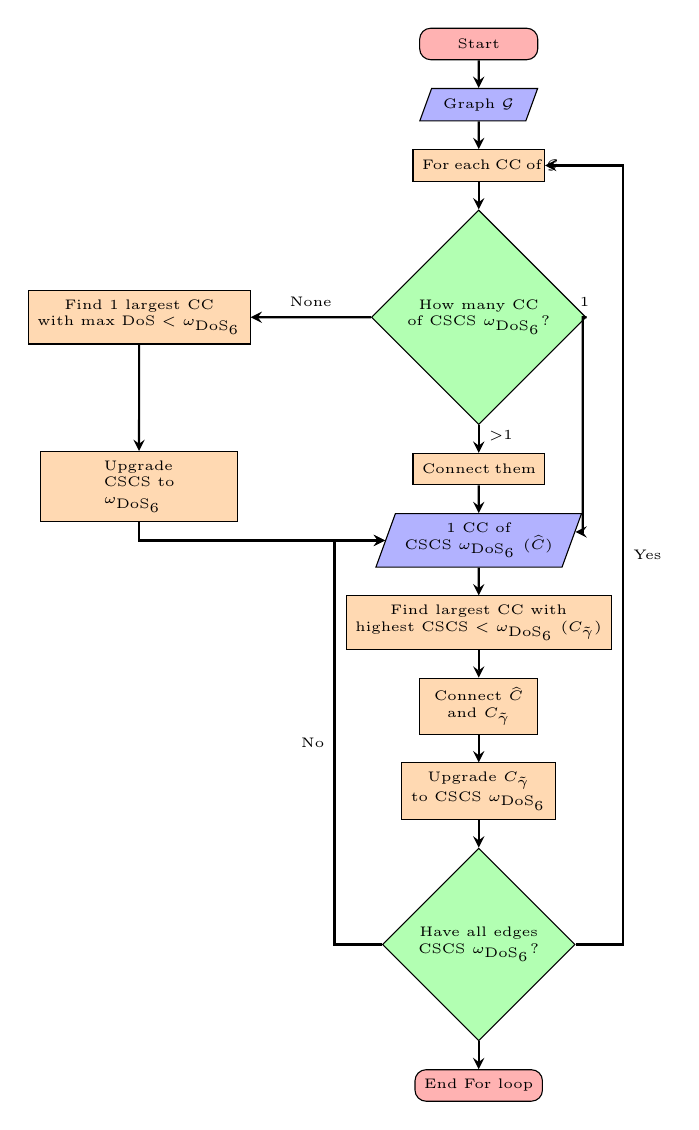
\begin{tikzpicture}[scale=0.6] % Scale down the entire TikZ picture
        \tikzstyle{label} = [font=\tiny] % Smaller font size
        \tikzstyle{default} = [%
        label,align=center, text centered, draw=black,
        execute at begin node={\begin{varwidth}{6em}}, % Reduced varwidth
        minimum height=0.4cm, % Reduced minimum height
        minimum width=1.5cm, % Reduced minimum width
        execute at end node={\end{varwidth}}]
        \tikzstyle{startstop} = [default, rectangle, rounded corners, fill=red!30]
        \tikzstyle{io} = [default, trapezium, trapezium left angle=70, trapezium right angle=110, fill=blue!30]
        \tikzstyle{process} = [default, rectangle, fill=orange!30, text centered] % Added text centered
        \tikzstyle{decision} = [default, diamond, fill=green!30, text centered] % Added text centered
        \tikzstyle{arrow} = [label, thick,->,>=stealth, font=\tiny] % Smaller font size

        \node[startstop] (start) {Start};
        \node[io, below=1em of start] (input-g) {Graph $\mathcal{G}$}; % Reduced spacing
        \draw[arrow] (start) -- (input-g) {};
        
        \node[process, below=1em of input-g] (for-each) {For each CC of $\mathcal{G}$}; % Reduced spacing
        \draw[arrow] (input-g) -- (for-each) {};
        
        \node[decision, below=1em of for-each] (number-dos-6) {How many CC\\of CSCS $\omega_{\text{DoS}_6}$?}; % Reduced spacing
        \draw[arrow] (for-each) -- (number-dos-6) {};
        
        \node[process, left=of number-dos-6, xshift=-1.5em] (largest-cc-sub-dos) {Find 1 largest CC\\with max DoS < $\omega_{\text{DoS}_6}$}; % Adjusted position and spacing
        \draw[arrow] (number-dos-6) -- (largest-cc-sub-dos) node[pos=0.5, above] {None};
      \node[process, below=of largest-cc-sub-dos, yshift=-1em, text centered, minimum height=0.5cm, minimum width=2.5cm] (upgrade-sub-dos) {\begin{varwidth}{1.5cm} Upgrade CSCS to $\quad \quad  \quad \omega_{\text{DoS}_6}$  \end{varwidth}};% Adjusted position and spacing
        \draw[arrow] (largest-cc-sub-dos) -- (upgrade-sub-dos);
        
        \node[process, below=1em of number-dos-6] (connect-cc-6) {Connect them}; % Reduced spacing
        \draw[arrow] (number-dos-6) -- (connect-cc-6) node[pos=0.4, right] {>1};

        \node[io, below=1em of connect-cc-6] (fuse) {1 CC of\\CSCS $\omega_{\text{DoS}_6}$ ($\widehat{C}$)}; % Reduced spacing
        \draw[arrow] (upgrade-sub-dos) |- (fuse) {};
        \draw[arrow] (connect-cc-6) -- (fuse) {};
        \draw[arrow] (number-dos-6) -- node[pos=0.5, above] {1} ++(2.2,0) |- (fuse.5);

        \node[process, below=1em of fuse] (find-max-sub-cc) {Find largest CC with\\highest CSCS < $\omega_{\text{DoS}_6}$ ($C_{\tilde{\gamma}}$)}; % Reduced spacing
        \draw[arrow] (fuse) -- (find-max-sub-cc) {};
        
        % Modified node to be larger and text centered
        \node[process, below=1em of find-max-sub-cc] (connect) {Connect $\widehat{C}$ \\and $C_{\tilde{\gamma}}$}; % Adjusted size
        \draw[arrow] (find-max-sub-cc) -- (connect) {};
        
        \node[process, below=1em of connect] (upgrade) {Upgrade $C_{\tilde{\gamma}}$\\to CSCS $\omega_{\text{DoS}_6}$}; % Reduced spacing
        \draw[arrow] (connect) -- (upgrade) {};
        
        \node[decision, below=1em of upgrade] (complete-edges) {Have all edges\\CSCS $\omega_{\text{DoS}_6}$?}; % Reduced spacing
        \draw[arrow] (upgrade) -- (complete-edges) {};

        % Adjusted arrow to avoid overlapping with specified nodes
        \draw[arrow] (complete-edges.east) -- ++(1,0) |- (for-each.east) node[pos=0.25, right] {Yes};
        \draw[arrow] (complete-edges.west) -- ++(-1,0) |- (fuse.west) node[pos=0.25, left] {No};

        \node[startstop, below=1em of complete-edges] (end) {End For loop}; % Reduced spacing
        \draw[arrow] (complete-edges) -- (end);
    \end{tikzpicture}
    \caption{\footnotesize Flowchart of the MLCC algorithm.}
    \label{tikz:flowchart-mlcc}
\end{figure}

% \onecolumn
% \section*{APPENDIX C}
% \label{Sioux_falls_analysis}
% \clearpage
\begin{figure*}[h!]
% \vspace{0.2cm}
%   \centering
\vspace{0.2cm}
\centering
\text{APPENDIX C} 

% Manually add title
% \\
% In Fig.~\ref{maximize_three_algorithms_sioux_falls}, we present the results of the MLCC algorithm for the Sioux Falls benchmark, while Table VIII shows the computational time for each algorithm.
\begin{minipage}{\textwidth}
\raggedright
\vspace{0.02\linewidth}
In Fig.~\ref{maximize_three_algorithms_sioux_falls}, we present the results of the optimization algorithms for the Sioux Falls benchmark, the evolution of the genetic algorithms and Table VIII shows the computational time for each one.
\end{minipage}
\vspace{0.3cm}  % Adjust spacing if needed
  \captionsetup[subfigure]{font={footnotesize}, labelfont={footnotesize, bf}, textfont={footnotesize, rm}}

  \subfloat[]{\includegraphics[width=0.95\linewidth]{Images/maximize_safety_academic_example_Sioux_Falls.png}\label{sf_1_r}} \\
  \subfloat[]{\includegraphics[width=0.42\linewidth]{Images/Sioux_Falls_comparation_GA_LCC_safety.png}\label{sf_2_r}}
  \hspace{0.03\linewidth}
  \subfloat[]{\includegraphics[width=0.40\linewidth]{Images/Grenoble_comparation_GA_LCC_safety_legend.png}\label{sf_3_legend}}

  \caption{\footnotesize (a) Results of solving Problem~$2$ using the MLCC, SGA, SGA-MLCC, and Bayesian algorithms on the Sioux Falls cycling network. The percentage improvement is calculated as \% = $|\hat{y}_{\omega_{0}} - \hat{y}(\omega^{\ast})| \times 100 / |\hat{y}_{FS} - \hat{y}_{\omega_0}|$. (b) show the performance evolution of the SGA and SGA-MLCC algorithms over generations for safety with (c) providing the legend. And $B_{\max} =$ 194,848€.}
\label{maximize_three_algorithms_sioux_falls}
  % Table inside figure environment
  \vspace{10pt} % Add vertical space between the figure and the table

  
   \begin{minipage}{\textwidth}
    \centering
    \captionsetup{labelformat=empty} % Temporarily empty label format
    \renewcommand{\thetable}{TABLE \arabic{table}} % Change table numbering
    \footnotesize
    \begin{tabular}{|c|c|c|c|c|c|c|c|c|c|c|}
    \hline
    \textbf{Algorithm} & \multicolumn{10}{|c|}{\textbf{Time}} \\ \hline
     & $i = 0$ & $i = 1$ & $i = 2$ & $i = 3$ & $i = 4$ & $i = 5$ & $i = 6$ & $i = 7$ & $i = 8$ & $i = 9$ \\ \hline
 MLCC & 0.08 s & 0.09 s & 0.08 s & 0.07 s & 0.08 s & 0.1 s & 0.1 s & 0.1 s & 0.14 s & 0.14 s \\ \hline
SGA & 25.66 s & 13.04 s & 12.98 s & 27.6 s & 14.74 s & 17.91 s & 29.0 s & 20.96 s & 23.4 s & 40.14 s\\ \hline
SGA-MLCC & 13.19 s & 12.54 s & 12.74 s & 15.07 s & 14.33 s & 15.63 s & 17.12 s & 20.12 s & 23.57 s & 27.32 s \\ \hline
Bayesian & 4.1 m & 4.03 m & 4.06 m & 5.34 m & 5.96 m & 6.01 m & 5.67 m & 5.69 m & 6.25 m & 6.42 m \\ \hline

%  & \multicolumn{10}{|c|}{\textbf{Comfort}} \\ \hline
 
%  MLCC & 0.2 s & 0.08 s & 0.08 s & 0.06 s & 0.08 s & 0.1 s & 0.1 s & 0.1 s & 0.14 s & 0.16 s \\ \hline
% SGA & 24.1 s & 11.41 s & 24.24 s & 13.33 s & 25.67 s & 15.56 s & 28.0 s & 19.43 s & 19.43 s & 36.1 s \\ \hline
% SGA-MLCC & 11.74 s & 11.67 s & 11.95 s & 13.54 s & 13.56 s & 15.63 s & 16.26 s & 17.68 s & 18.22 s & 25.61 s \\ \hline
% Bayesian & 3.8 m & 3.73 m & 3.83 m & 4.04 m & 5.96 m & 6.17 m & 5.93 m & 5.92 m & 6.02 m & 5.89 m \\ \hline
    \end{tabular}
    \caption{TABLE VIII: Calculation time for the Sioux Falls cycling network.}
    \label{sioux_falls_time_table}
  \end{minipage}
\end{figure*}
\FloatBarrier
% \afterpage{\twocolumn}
% \vspace{-30cm}
% \twocolumn
%--------------------------------------
% The pseudocode refers to the MLCC algorithm described in Section~\ref{section:mlcc}. Steps correspond to the different items.

% \floatname{algorithm}{Algorithm}
% \begin{algorithm}[ht]
% \caption*{MLCC Algorithm} 
% \label{edges_upgrade_pseudocode}
% \footnotesize
% \begin{algorithmic}[1]
% \State \textbf{Input:} Original graph: $\mathcal{G}$. Budget: $B$.
% \State \textbf{Output:} $\mathcal{G}$ with edges upgraded.
% \For{$C$ \textbf{in} set of CCs of $\mathcal{G}$}
% \algrule
% \State $\mathcal{G}_{C} \gets (V(\mathcal{G}_{C}), E(\mathcal{G}_{C}), W(\mathcal{G}_{C}))$ induced graph by $C$
% \State $\gamma \gets \max{ \left \{ \omega_{e} \colon e \in E(\mathcal{G}_{C}) \right \} }$
% \State list\_$\mathcal{G}_{C} \gets \left \{ C_{\gamma} \colon C_{\gamma} \text{ is a connected subgraph } \right.$
% \State $\quad $ (see Section~\ref{connected_component})  \Comment{{\color{gray} Step 1.1 }} 
% \State $C_{\hat{\gamma}} \gets \max{ \left \{ \text{list\_}\mathcal{G}_{C} \right \}}$
% \If{$\gamma < 6$}
%         \State Upgrade Subgraph($C_{\hat{\gamma}}, B$)
%     \EndIf
%     \algrule
% \If{$\gamma == \max{ \left \{ \omega_{e} \colon e \in E(C_{\hat{\gamma}}) \right \}}$}
%         \For{$C_{\tilde{\gamma}}$ \textbf{in} $\text{sorted(list\_}\mathcal{G}_{C}) $}
%         \State Connect Graphs($C_{\hat{\gamma}}, C_{\tilde{\gamma}}, B$) \Comment{{\color{gray} Step 1.2 }} 
% \EndFor
% \EndIf
% \algrule
% \For{$\tilde{\gamma} \gets 5$ \textbf{to} $2$}
%         \State $\text{list\_}\mathcal{G}_{C_{\tilde{\gamma}}} \gets \left \{ C_{\tilde{\gamma}} \colon C_{\tilde{\gamma}} \text{ is a connected subgraph} \right \}$ 
%         \State $\quad \quad \quad \quad \quad$ (see Section~\ref{connected_component})
%         \For{$C_{\tilde{\gamma}}$ \textbf{in} $\text{sorted(list\_}\mathcal{G}_{C_{\tilde{\gamma}}})$} \Comment{{\color{gray} Step 2 }} 
%         \State Connect Graphs ($C_{\hat{\gamma}}, C_{\tilde{\gamma}}, B$) 
%         \State Upgrade Subgraph($C_{\tilde{\gamma}}, B$)
% \EndFor
% \EndFor
% \algrule
% \EndFor
% \end{algorithmic}
% \end{algorithm}
%--------------------------------------
%Connected graphs $C_{\gamma}$ and $C_{\tilde{\gamma}}$ are constructed using the same criteria as defined in the $l_{\mathcal{G}}$ metric. They are sorted to arrange their elements in descending order based on the total geographical length of their edges.


% \floatname{algorithm}{Function}
% \begin{algorithm}[H]
% \caption*{Connect Graphs}
% \label{pseudocode:connect_graphs}
% \footnotesize
% \begin{algorithmic}[1]
% \State \textbf{Input:} Graphs: $\mathcal{G}_{1}$ and $\mathcal{G}_{2}$. Budget: $B$.
% \State \textbf{Output:} Upgrade the DoS of DoS shortest path between $\mathcal{G}_{1}$ and $\mathcal{G}_{2}$ so that all its edges have the maximum possible DoS value.
% \For{$e$ \textbf{in} shortest DoS path between $\mathcal{G}_{1}$ and $\mathcal{G}_{2}$}
% \For{$i \gets 6$ \textbf{to} $2$}
%     \If{$B \geq d_{e} \cdot \pi(\omega_{e}, i)$ \textbf{and} $i > \omega_{e}$}
%         \State $\omega_{e} \gets i$
%         \State $B \gets B-d_{e} \cdot \pi(\omega_{e}, i)$
%     \Else
%         \State \textbf{end Main Algorithm}
%     \EndIf
% \EndFor
% \EndFor
% \end{algorithmic}
% \end{algorithm}

% \floatname{algorithm}{Function}
% \begin{algorithm}[H]
% \caption*{Upgrade Subgraph}
% \label{pseudocode:upgrade_subpgraph}
% \footnotesize
% \begin{algorithmic}[1]
% \State \textbf{Input:} Subgraph: $\mathcal{H}$. Budget: $B$.
% \State \textbf{Output:} $\mathcal{H}$ with edges upgraded at the maximum possible DoS value.
% \For{$e$ \textbf{in} edges of $\mathcal{H}$}
% \For{$i \gets 6$ \textbf{to} $2$}
%     \If{$B \geq d_{e} \cdot \pi(\omega_{e}, i)$ \textbf{and} $i > \omega_{e}$}
%         \State $\omega_{e} \gets i$
%         \State $B \gets B-d_{e} \cdot \pi(\omega_{e}, i)$
%     \Else
%         \State \textbf{end Main Algorithm}
%     \EndIf
% \EndFor
% \EndFor
% \end{algorithmic}
% \end{algorithm}

%--------------------------------------




\bibliographystyle{unsrt}
\bibliography{labiblio}
% \newpage

% \vspace{11pt}
%--------------------------------------
% Biography section
\begin{IEEEbiography}[{\includegraphics[width=1in,height=1.25in,clip,keepaspectratio]{Images/MCJ.pdf}}]{Manuel Campero Jurado}
received the B.S. degree in applied mathematics in 2019 and the M.S. in 2021 degree in mathematics from the Autonomous University of the State of Hidalgo, Mexico. He is currently
pursuing the PhD. degree from the Grenoble Institute of Technology, Grenoble, France. His research interests include modeling and optimization of safety networks for cyclists.
\end{IEEEbiography}
\vspace{0cm}
\begin{IEEEbiography}[{\includegraphics[width=1in,height=1.25in,clip,keepaspectratio]{Images/CCDW.pdf}}]{Carlos Canudas de Wit}
% received the B.S. degree in electronics and communications from the Monterrey Institute of Technology and Higher Education, Monterrey, Mexico, in 1980, and the M.S. and Ph.D. degrees in automatic control from the Grenoble Institute of Technology, Grenoble, France, in 1984 and 1987, respectively. He is currently a Directeur de recherche (Senior Researcher) with CNRS, Grenoble, France, where he is the Leader with the NeCS Team, a joint team of GIPSA-Lab (CNRS) and INRIA, on networked controlled systems. Dr. Canudas-de-Wit is an IFAC Fellow. He was an Associate Editor of the IEEE Transactions on Automatic Control, Automatica, and IEEE Transactions on Control Systems Technology. He is an Associate Editor of the Asian Journal of Control, and the IEEE Transactions on Control of Network Systems. He served as the President of the European Control Association from 2013 to 2015, and a member of the IEEE Board of Governors of the Control System Society from 2011 to 2014. He holds the ERC Advanced Grant Scale-FreeBack from 2016 to 2021. His research interests include Electric Vehicles, Optimal Control, Traffic Model and Large-scale Networks.
received his B.S. in electronics and communications from the Monterrey Institute of Technology, Mexico, in 1980, and his M.S. and Ph.D. in automatic control from the Grenoble Institute of Technology, France, in 1984 and 1987, respectively. He is a Directeur de recherche (Senior Researcher) at CNRS, Grenoble, leading the NeCS Team (GIPSA-Lab \& INRIA) on networked controlled systems. An IFAC Fellow, he has served as Associate Editor for multiple IEEE journals and was President of the European Control Association (2013–2015). He held the ERC Advanced Grant Scale-FreeBack (2016–2021). His research focuses on electric vehicles, optimal control, traffic modeling, and large-scale networks.
\end{IEEEbiography}
\vspace{0cm}
\begin{IEEEbiography}[{\includegraphics[width=1in,height=1.25in,clip,keepaspectratio]{Images/GDN.pdf}}]{Giovanni De Nunzio}
received the B.S. and M.S. degrees in information and automation engineering from the University of L’Aquila, Italy, in 2007 and 2010, respectively, and the Ph.D. degree in automatic control from the Grenoble Institute of Technology (Grenoble INP), France, in 2015. He is currently a Research Engineer and an Research and Innovation Project Leader with IFP Energies nouvelles, Lyon, France. His research activities focus on modeling and control of transportation and mobility systems, advanced driver-assistance systems, graph theory, optimization, and data science.
\end{IEEEbiography}


\end{document}


The pseudocode refers to the MLCC algorithm described in Section~\ref{section:mlcc}. Steps correspond to the different items.

\floatname{algorithm}{Algorithm}
\begin{algorithm}[ht]
\caption*{MLCC Algorithm} 
\label{edges_upgrade_pseudocode}
\footnotesize
\begin{algorithmic}[1]
\State \textbf{Input:} Original graph: $\mathcal{G}$. Budget: $B$.
\State \textbf{Output:} $\mathcal{G}$ with edges upgraded.
\For{$C$ \textbf{in} set of CCs of $\mathcal{G}$}
\algrule
\State $\mathcal{G}_{C} \gets (V(\mathcal{G}_{C}), E(\mathcal{G}_{C}), W(\mathcal{G}_{C}))$ induced graph by $C$
\State $\gamma \gets \max{ \left \{ \omega_{e} \colon e \in E(\mathcal{G}_{C}) \right \} }$
\State list\_$\mathcal{G}_{C} \gets \left \{ C_{\gamma} \colon C_{\gamma} \text{ is a connected subgraph } \right.$
\State $\quad $ (see Section~\ref{connected_component})  \Comment{{\color{gray} Step 1.1 }} 
\State $C_{\hat{\gamma}} \gets \max{ \left \{ \text{list\_}\mathcal{G}_{C} \right \}}$
\If{$\gamma < 6$}
        \State Upgrade Subgraph($C_{\hat{\gamma}}, B$)
    \EndIf
    \algrule
\If{$\gamma == \max{ \left \{ \omega_{e} \colon e \in E(C_{\hat{\gamma}}) \right \}}$}
        \For{$C_{\tilde{\gamma}}$ \textbf{in} $\text{sorted(list\_}\mathcal{G}_{C}) $}
        \State Connect Graphs($C_{\hat{\gamma}}, C_{\tilde{\gamma}}, B$) \Comment{{\color{gray} Step 1.2 }} 
\EndFor
\EndIf
\algrule
\For{$\tilde{\gamma} \gets 5$ \textbf{to} $2$}
        \State $\text{list\_}\mathcal{G}_{C_{\tilde{\gamma}}} \gets \left \{ C_{\tilde{\gamma}} \colon C_{\tilde{\gamma}} \text{ is a connected subgraph} \right \}$ 
        \State $\quad \quad \quad \quad \quad$ (see Section~\ref{connected_component})
        \For{$C_{\tilde{\gamma}}$ \textbf{in} $\text{sorted(list\_}\mathcal{G}_{C_{\tilde{\gamma}}})$} \Comment{{\color{gray} Step 2 }} 
        \State Connect Graphs ($C_{\hat{\gamma}}, C_{\tilde{\gamma}}, B$) 
        \State Upgrade Subgraph($C_{\tilde{\gamma}}, B$)
\EndFor
\EndFor
\algrule
\EndFor
\end{algorithmic}
\end{algorithm}
%Connected graphs $C_{\gamma}$ and $C_{\tilde{\gamma}}$ are constructed using the same criteria as defined in the $l_{\mathcal{G}}$ metric. They are sorted to arrange their elements in descending order based on the total geographical length of their edges.


\floatname{algorithm}{Function}
\begin{algorithm}[H]
\caption*{Connect Graphs}
\label{pseudocode:connect_graphs}
\footnotesize
\begin{algorithmic}[1]
\State \textbf{Input:} Graphs: $\mathcal{G}_{1}$ and $\mathcal{G}_{2}$. Budget: $B$.
\State \textbf{Output:} Upgrade the DoS of DoS shortest path between $\mathcal{G}_{1}$ and $\mathcal{G}_{2}$ so that all its edges have the maximum possible DoS value.
\For{$e$ \textbf{in} shortest DoS path between $\mathcal{G}_{1}$ and $\mathcal{G}_{2}$}
\For{$i \gets 6$ \textbf{to} $2$}
    \If{$B \geq d_{e} \cdot \pi(\omega_{e}, i)$ \textbf{and} $i > \omega_{e}$}
        \State $\omega_{e} \gets i$
        \State $B \gets B-d_{e} \cdot \pi(\omega_{e}, i)$
    \Else
        \State \textbf{end Main Algorithm}
    \EndIf
\EndFor
\EndFor
\end{algorithmic}
\end{algorithm}

\floatname{algorithm}{Function}
\begin{algorithm}[H]
\caption*{Upgrade Subgraph}
\label{pseudocode:upgrade_subpgraph}
\footnotesize
\begin{algorithmic}[1]
\State \textbf{Input:} Subgraph: $\mathcal{H}$. Budget: $B$.
\State \textbf{Output:} $\mathcal{H}$ with edges upgraded at the maximum possible DoS value.
\For{$e$ \textbf{in} edges of $\mathcal{H}$}
\For{$i \gets 6$ \textbf{to} $2$}
    \If{$B \geq d_{e} \cdot \pi(\omega_{e}, i)$ \textbf{and} $i > \omega_{e}$}
        \State $\omega_{e} \gets i$
        \State $B \gets B-d_{e} \cdot \pi(\omega_{e}, i)$
    \Else
        \State \textbf{end Main Algorithm}
    \EndIf
\EndFor
\EndFor
\end{algorithmic}
\end{algorithm}



